\documentclass[12pt,a4paper,titlepage]{article}
\usepackage{License_style}

% the document should be compiled with pdfLaTex

\begin{document}

% \numberwithin{lstlisting}{section}

\phantomsection

%##############################################################################

% WikiBooks (http://en.wikibooks.org/wiki/LaTeX/Title_Creation)
%
% License:
% CC BY-NC-SA 3.0 (http://creativecommons.org/licenses/by-nc-sa/3.0/)
% 
% Instructions for using this template:
% This title page is capable of being compiled as is. This is not useful for 
% including it in another document. To do this, you have two options: 
%
% 1) Copy/paste everything between \begin{document} and \end{document} 
% starting at \begin{titlepage} and paste this into another LaTeX file where you 
% want your title page.
% OR
% 2) Remove everything outside the \begin{titlepage} and \end{titlepage} and 
% move this file to the same directory as the LaTeX file you wish to add it to. 
% Then add \input{./title_page_1.tex} to your LaTeX file where you want your
% title page.
%
%%%%%%%%%%%%%%%%%%%%%%%%%%%%%%%%%%%%%%%%%

%----------------------------------------------------------------------------------------
%	PACKAGES AND OTHER DOCUMENT CONFIGURATIONS
%----------------------------------------------------------------------------------------




\begin{titlepage}

\newcommand{\HRule}{\rule{\linewidth}{0.5mm}} % Defines a new command for the horizontal lines, change thickness here

\center % Center everything on the page
 
%----------------------------------------------------------------------------------------
%	HEADING SECTIONS
%----------------------------------------------------------------------------------------

Ministerul Educatiei al Republicii Moldova\\ % Name of your university/college
\textbf{Universitatea Tehnica a Moldovei}\\% Name of your university/college
Facultatea de Calculatoare, Informatica și Microelectronica\\
Filiera Anglofona "Computer Science"\\


\vspace{2cm}



\hfill Admis la sustinere\\
\hfill Sef de catedra: prof. dr. hab. Viorel Bostan\\

\vspace{0.4cm}
\hfill "\rule{0.75cm}{0.2mm}" \ \rule{3cm}{0.2mm} 2015
\vspace{3cm}




\begin{center}
\Large \textbf{Monitoring Application for Courses}\\
\vspace{0.6cm}
Proiect de licență
\end{center}
\vspace{1cm}


\hfill Student: \rule{3.9cm}{0.2mm}(A.Plesco)\\
\vspace{0.2cm}
\hfill Conducator: \rule{4cm}{0.2mm}(M.Balan)\\
\vspace{0.2cm}
\hfill Consultanti: \rule{4.2cm}{0.2mm}(I.Tyrell)\\
\vspace{0.2cm}
\hfill \rule{4cm}{0.2mm}(G.Covdii)\\
\vspace{0.2cm}
\hfill \rule{3.9cm}{0.2mm}(V.Bostan)\\
\vspace{0.2cm}
\hfill \rule{4cm}{0.2mm}(M.Balan)\\
\vspace{4cm}



% If you don't want a supervisor, uncomment the two lines below and remove the section above
%\Large \emph{Author:}\\
%John \textsc{Smith}\\[3cm] % Your name

%----------------------------------------------------------------------------------------
%	DATE SECTION
%----------------------------------------------------------------------------------------
\begin{center}
Chisinau 2015
\end{center}
%{\large \today}\\[3cm] % Date, change the \today to a set date if you want to be precise

%----------------------------------------------------------------------------------------
%	LOGO SECTION
%----------------------------------------------------------------------------------------

%\includegraphics{Logo}\\[1cm] % Include a department/university logo - this will require the graphicx package
 
%----------------------------------------------------------------------------------------

\vfill % Fill the rest of the page with whitespace

\end{titlepage}



\cleardoublepage

\section*{Abstract}
Thesis \textbf{Using Semantic Analysis of Moldovan Online Media as a Way to Reveal Patterns and Trends} presented by Terman Sergiu was written in English. It has 25 figures, 11 listings, 8 tables, and 15 references. The report consists of introduction, 4 chapters, and conclusions.

The thesis aims to research the potential of data journalism in Republic of Moldova. For that purpose, OpenMedia project was developed. It is a platform that aggregates online media channels for offering means of visualization of word frequency requested by a user.

The application was build using Ruby programming language. The platform consists from two components. The first one is the data gathering and preprocessing. It can be divided in four smaller parts. Crawling the media channels an fetching the article pages, parsing the articles and storing to database, executing natural language processing operations over articles and preparing data for client side visualization. The second part of the platform is the client side application. It aims to provide an interactive way for querying words and visualizing the data. The data representation is done using enhanced line plots that denote the word frequency for different media sources.

The technologies used are Sinatra framework for building the web interface, MongoDB for storing the data and running native mapreduce tasks, Sidekiq for launching asynchronous jobs and Racai SOAP service for NLP operations.

OpenMedia represents an attempt to offer a tool for data journalism targeted for Republic of Moldova. It does not have many features but it has the right infrastructure for future development. It also proved that a data journalism software has a lot of potential on inexistent local market.
\clearpage

\section*{Rezumat}
Lucrarea \textbf{Utizitarea analizei semantice a online media din Moldova, pentru detectarea tendințelor si modelelor} prezentată de Terman Sergiu a fost scrisă în engleză. Ea constă din 25 de figuri, 11 secvențe de cod, 8 tabele și 15 referințe. Lucrarea face parte din introducere, 4 capitole și concluzii.

Teza are ca scop cercetarea potențialului jurnalismului pe bază de date în Republica Moldova. Prin urmare proiectul OpenMedia a fost dezvoltat. Aceasta este o platformă care agreghează canalele media disponibile online, pentru a oferi mijloace de vizualizare a frecvenței menționării a unui cuvânt specificat de către utilizator.

Aplicația a fost dezvoltată utilizând limbajul de programare Ruby. Platforma consită din două părți. Prima parte reprezinta adunarea și preprocesarea datelor. Aceasta poate fi divizată în patru entități. Accesarea canalelor media și descărcarea articolelor, parsarea fișierelo descărcate pentru a extrage conținutul textual al articolelor și salvarea lor în bază de date, aplicarea operațiilor de procesare a limbajului natural, pregătirea datelor pentru a fi vizualizate. A doua parte a platformei reprezintă aplicația utilizatorului. Aceasta are drept obiectiv să ofere o modalitate interactivă de interogare a cuvintelor și vizualizare a datelor. Reprezentarea datelor este realizată prin intermediul graficilor liniare ce denotă frecvența cuvântului în cadrul diferitor surse media.

Tecnologiile utilizate sunt următoarele. Sinatra framework pentru dezvoltarea interfeței web. Baza de date folosită este MongoDB. Aplicația Sidekiq este folosită pentru lansarea sarcinilor \mbox{asincrone}. Serviciul Racai este folosit pentru executarea operațiunilor de procesare a limbajului \mbox{natural}.


OpenMedia reprezintă o încercare de a oferi un instrument de jurnalism pe bază de date, orientată pentru Republica Moldova. Ea nu cuprinde multe funcționalități la nivelul utilizatorului, însă are infrastructura necesară pentru o dezvoltare în viitor. Acest proiect a demonstat faptul că așa un instrument are un mare potențial pe piață locală, fiind pioner în acest domeniu.

\clearpage

\tableofcontents
\addtocontents{toc}{\protect\thispagestyle{empty}} % no page number on the table of contents page
\cleardoublepage

\listoffigures
\addcontentsline{toc}{section}{List of figures}
\clearpage

\lstlistoflistings
\addcontentsline{toc}{section}{Listings}
\thispagestyle{empty}
\clearpage

% ABREVIERI. Este recomandabila doar daca utilizezi in text peste 10-15 abrevieri
\phantomsection
\addcontentsline{toc}{section}{Abbreviations}
\section*{Abbreviations}

\begin{itemize}[leftmargin=2cm, topsep=0pt, partopsep=5pt,itemsep=0pt,parsep=0pt]
\item[HTTP --] HyperText Transfer Protocol
\item[HTTPS --] Secure HyperText Transfer Protocol
\item[TLS --] Transport Layer Security
\item[SSL --] Secure Sockets Layer
\item[HTML --] HyperText Markup Language
\item[XML --] Extensible Markup Language
\item[JSON --] Java Script Object Notation
\item[NLP --] Natural Language Processing
\item[REST --] Representational state transfer
\item[SOAP --] Simple Object Access Protocol
\item[WSDL --] Web Services Description Language
\item[RPC --] Remote procedure call
\item[DCOM --] Distributed Component Object Model
\item[CORBA --] Common Object Request Broker Architecture
\item[RMI --] Remote method invocation
\item[XSD --] XML Schema Definition
\item[SMTP --] Simple Mail Transfer Protocol
\item[CRUD --] Create Read Update Delete
\item[URI --] Uniform Resource Identifier
\item[URL --] Uniform Resource Locator
\item[RFC --] Request for Comments
\item[API --] Application Programming Interface
\item[HATEOAS --] Hypertext As The Engine Of Application State
\item[CAR --] Computer Assigned Reporting
\item[TCP --] Transmission Control Protocol
\item[UX --] User Experience
\item[AJAX --] Asynchronous JavaScript and XML
\item[DOM --] Document Object Model
\item[UI --] User Interface
\item[MVC --] Model View Controller
\item[BI --] Business Intelligent
\item[RDBMS --] Relational database management system
\item[SQL --] Structured Query Language
\item[ACID --] Atomicity, Consistency, Isolation, Durability
\item[BASE --] Basically Available, Soft state, Eventual consistency
\item[CAP --] Consistency Availability Network Partition tolerance
\item[DBMS --] Database Management System
\item[ORM --] Object Relational Mapping
\end{itemize}
\thispagestyle{empty}
\cleardoublepage

%INTRODUCERE
%\setcounter{page}{17}
\phantomsection
\addcontentsline{toc}{section}{Introduction}
\section*{Introduction}
\phantomsection
A continuous stream of information is daily consumed by a person. It is represented in different forms under various formats. And due to the great amounts of data that surrounds us nowadays, communication efficiency became a crucial problem. Throughout the time, data representation suffered a sequence of changes, thus constantly evolving. Starting from architecture, letters on papers ending with radio, television and computers wired through Internet.

Textual format remains the most common method of transmitting information. Though not the most efficient, it is cheap in terms of storage, expressive and extensive. The problem is that people encounter problems in the process of absorbing textual data. The mnemonic techniques usually are not enough for extracting the key information from text.

Text processing on a bigger scale becomes a tedious operation for a human being. That's why people resort to computers in order to solve the problem more efficiently. Data Science, a fairly new field in computer science, tackles this problem. Actually it employs techniques and theories drawn from many fields within the broad areas of mathematics, statistics, information theory, probability models, machine learning, data mining, database, pattern recognition and many others. The problems which it solves are marketing optimization, fraud detection, trends detection even bets.

The problem researched in this work is concerning online media, articles published by Moldavian sources such as Timpul, Unimedia, Publika. The goal is to create a platform where users could query word frequency. Search for the trends relevant for different periods of time. Observe which sources are emphasizing specific key words, detect biases. Basically provide a visualization methods from which viable conclusions can be drawn. Why it is important to have such tool on the local market? Because there isn't one present. And second is that people running business, from various areas, could tune their approach based on results provided by platform. Journalism is another niche targeted by the platform. It is not that easy to write an article regarding events which happened in the course of an year. While it is much simpler when you can observe things like: when was a specific topic more popular and when it started to become less known. Which political entity is more discussed, in what period of time? News media is the quintessential origin of information feed. The good thing is that it can be processed and used, in terms of software, for providing data in an understandable manner.

The application would consist from two separate parts. First one represents the data mining platform. It have the purpose to go through media web portals and pull all the available articles. Extracts the articles content and store into a database. Run tokenization and part of speech tagger tasks in order to enrich the articles with useful metadata, used for meaningful queries and proper data visualization. The second part represents the client interaction application. its a web platform which provides querying features and visualization options. The queries most likely will represent map reduce tasks which will run on the storage used by the first platform. The communication bridge between the applications components is the database.

\clearpage
\cleardoublepage

% CAPITOLUL 1
\section{Project analysis and System requirements}
\phantomsection

\subsection{Problem Definition}
The platform OpenMedia is a rather complex system consisting from several parts. That is why is crucial to break it into smaller modules and logical components that can communicate with each other. There are lots of parts which the application should consist of: data fetching, cleaning the articles and enriching them with proper metadata, interactive modern web application, efficiently storing the data, running tasks independently, communication between system components, how to implement asynchronous messaging between modules, smart visualization of the data, what are the dependencies of some specific technologies, how this dependencies will co-work in combination with the rest of the system. If looked from a bigger scale the problem is not that simple, that's why a deeper level of structured granularity is required.

\subsection{Project Analysis}
The project OpenMedia is a platform used to provide visual models and statistic result based on online media sources from Republic of Moldova. It aims to collect the available articles found on the public sources and use them as a generic source for extracting useful results to be provided to visualization tools. The features offered by OpenMedia will be tools for querying for the desired keywords, in order to construct frequency plots, with options to see to what sources it belongs to. Also it will bring trend detection utilities. By selecting a range of time, it will render the most mentioned terms, and construct bar charts thus communicating the relevance of the popularity.

The platform will consist from two major parts.
\begin{itemize}
    \item Data gathering platform
    \begin{itemize}
        \item Fetching the article pages
        \item Extracting the article
        \item Storing the article
        \item Enriching with textual metadata
    \end{itemize}
    \item Web Client platform
    \begin{itemize}
        \item A simple and intuitive design
        \item Launching asynchronous tasks
        \item Receiving the finished
        \item Visualization of results
    \end{itemize}
\end{itemize}

\subsubsection{Data gathering platform}
This part of the application is focused on gathering data, cleaning and baking it. Simply put, all the heavy lifting of textual data preprocessing is done by this part of the platform. In the figure \ref{data_gathering_mock} is mocked the activity layers of the application. It is important to deliver the data in a format easily operable by the application because the amount of data analysis tricks becomes more various. To be more specific, it is up to client platform to choose the techniques of data consumption. On the one hand it does not sound as an optimized solution but on the other hand it offers flexibility. Data collection is a long and tedious process, that is why it should be better run once. More than that it is advised that all the data changes should be managed in a separate copy. Keeping each stage of data in an immutable state is a wise move. Redundancy is a better choice due to the fact that a project is prone to changes. Running the entire gathering operation from the bottom just in order to add a new feature sounds lethal to a business solution. That is why the OpenMedia platform saves each stage of data.

The articles used by the platform are the public sources of the online media of Republic of Moldova. These are Unimedia, Timpul and Publika. As a future goal is intended to include the other available resources, in order to make the platform more media agnostic. Adding to the system as many resources as possible is a key part of OpenMedia philosophy. The idea is that media sources are usually biased usually by political reasons, meaning that a research in a political area could lead to a less viable result. Beyond that the platform would provide means to deduce predispositions to some governmental parties.



\begin{figure}[!ht]
\centering
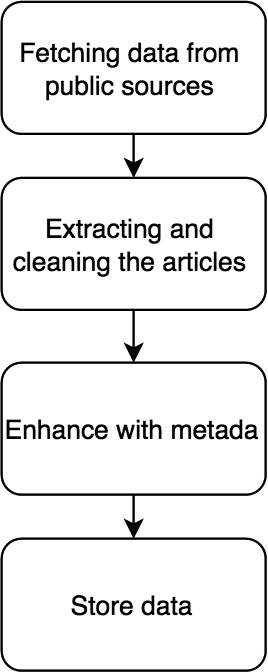
\includegraphics[width=3.8cm]{1_data_gathering}
\caption{Data Gathering platform mockup}\label{data_gathering_mock}
\end{figure}

\subsubsection{Web Client platform}
The client side will represent a web application, a minimalistic layer used for communication between user and the platform. Having a web infrastructure offers the opportunity to make the application easy to access. The only requirement being a modern web browser like Google Chrome, Firefox etc. The focus of the application is to make available the following functionalities.
\begin{itemize}
    \item execute queries on specified words
    \item execute trend detection queries on specified date rang
    \item display frequency line charts
    \item display trends popularity bar charts
\end{itemize}

This are the basic functionalities provided by the client application. Of course here are also included details such as specifying the media resource, in order to be able to compare the results and extract some useful conclusions from it. The goal is to make the user experience as natural as possible. And due to the fact that he number of functionalities are not so various, creating a natural flow of events will not represent an essential problem. But it should be taken into consideration that a reduced amount of functionalities does not mean a reduced amount of operations. The whole sequence of events is rather complex. It will be described step by step in the next pages of the report.

\begin{figure}[!ht]
\centering
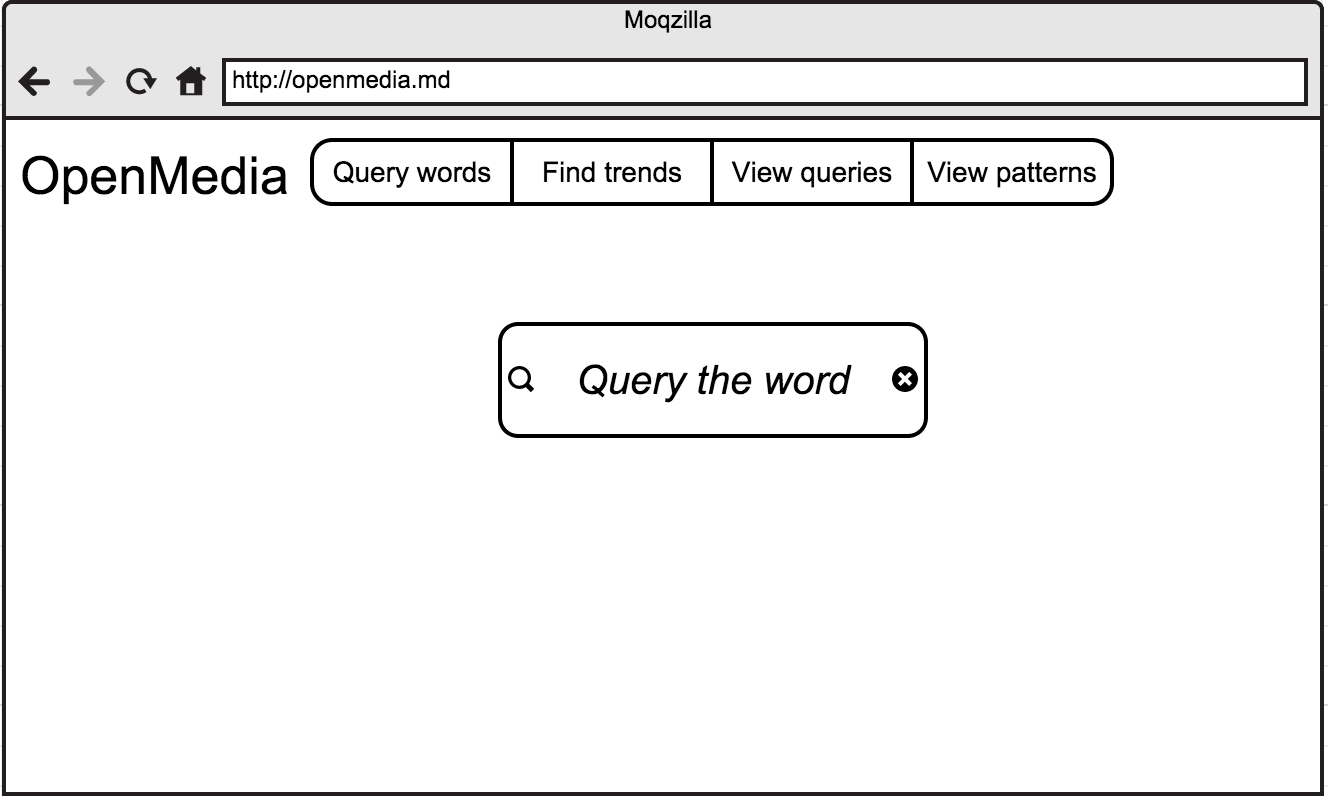
\includegraphics[width=13cm]{1_app_mock_1}
\caption{Primary page view}\label{app_mock_1}
\end{figure}

In order to make an expected view of the application. There are presented some mockups of the web applications. In figure \ref{app_mock_1} is represented the main page. The user has the input box used to execute queries related to word frequency. Because the query execution latency is going to be pretty long, the application is intended to work in an asynchronous way. So after the clicking, a notification will pop up informing that a query was started. Also a pop up notification will be displayed when there are news about the result. After which the result can accessed by clicking on View Queries button. By selecting the specific word, application is transitioning to a result view. The mockup of the page can be observed in figure \ref{1_app_mock_2}. A  plot is rendered representing the intensity per month which the word was mentioned. According to date range, the necessary conclusions be drawn. For example when was the specific word at it's peak. When it started to become less popular, what are the spikes, what caused the spikes. This might prove quite valuable information if examined from the right angle. The good part that anyone interested of statistic results can use it. Starting from business entrepreneurs which are trying to research the trendiness of a specific product, a journalist which is interested in popularity of a specific event or entity. The great part about it is that a personal set of queries can be done, thus building a custom aggregation of analytical results

\begin{figure}[!ht]
\centering
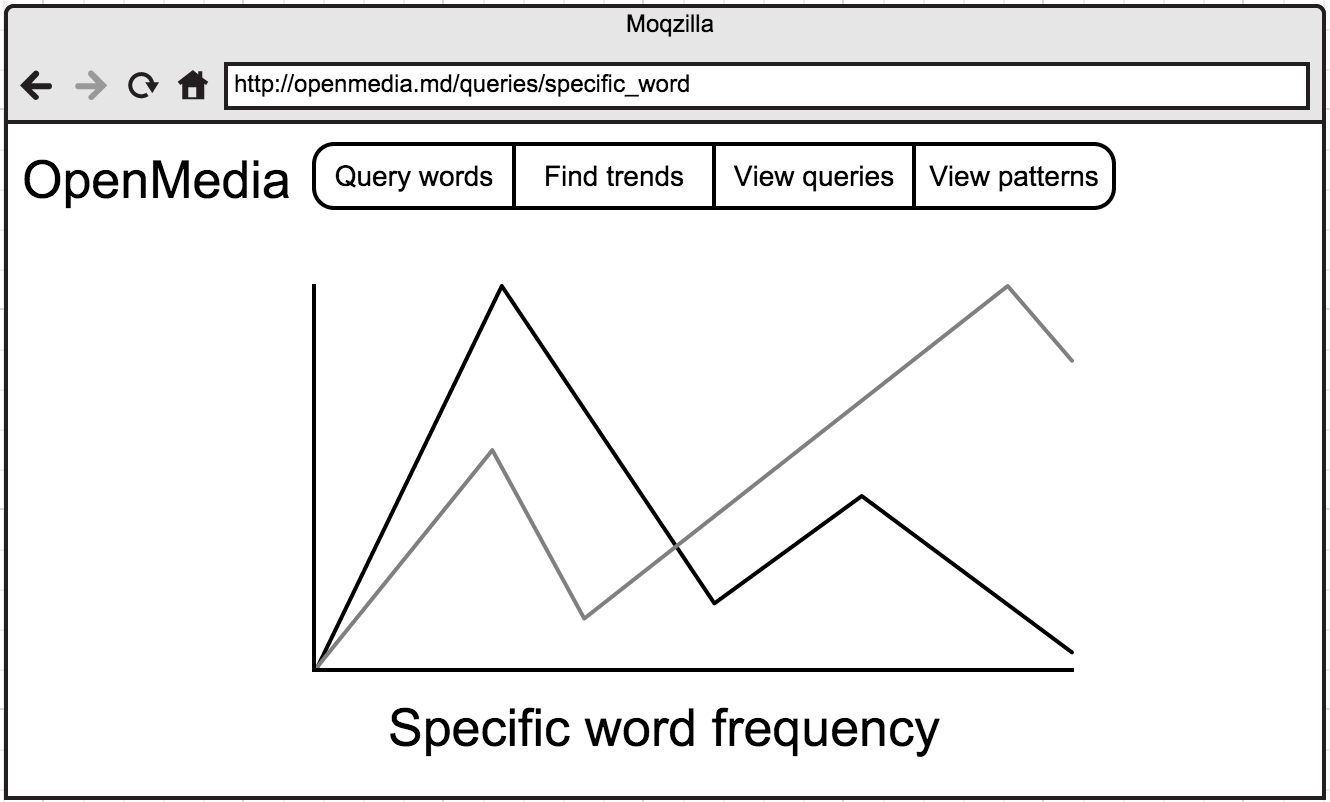
\includegraphics[width=13cm]{1_app_mock_2}
\caption{Frequency plot view}\label{app_mock_2}
\end{figure}

\subsection{Theoretical analysis}
Considering the complexity of the platform, a right amount of research is required in order to construct a workable product. The project OpenMedia consists of two independent separate product. Because both make part of the same new evolving field, data science, the final product represents a usable product which can be used on a local scale. Now will follow a more detailed description of various aspects of the platform, regarding the technologies best suited for building the application, the concepts involved under the hood, means of solving some specific problems.

\subsubsection{Modern Web Application}
Web applications are heavily using HTTP protocol as means of transporting the data. The thing is that HTTP is a stateless protocol. For every request made by a client a TCP socket is opened. The HTTP server is receiving the request and handled by the application layer which does the response decision. When the response is sent back to the client, the TCP socket is closed and the transaction ends. The whole chain of events is repeated basically at every user interaction. In the result the web application is becoming a stateless application itself. At least that was valid until concept of Web 2.0 was introduced in 2004. Java Script started to become more popular because it gave the power to animate the pages and create a more humane UX. But the magic was behind the AJAX technology. The concept introduced by AJAX was making a web page run asynchronous requests and make live partially DOM changes. Developers could create web applications which did not require full page reload at while interacting with the page. Successfully implementation of this concepts are Facebook, Gmail, Twitter etc. AJAX, JQuery and other Java Script technologies brought web applications one step closer to the desktop applications experience.

What is targeted now are the single page applications. The main reason is that they are able to offer more native application like experience to the user. This is hard to do with other approaches. Supporting rich interactions with multiple components on a page means that those components have many more intermediate states. Server side rendering is hard to implement for all the intermediate states. Small view states do not map well to URLs.

Single page applications are distinguished by their ability to redraw any part of the UI without requiring a server round trip to retrieve HTML. This is achieved by separating the data from the presentation of data by having a model layer that handles data and a view layer that reads from the models. Interaction with the single page application often involves dynamic communication with the web server behind the scenes.

Here are enumerated a set of popular technologies which offers the possibility of building single page applications:
\begin{itemize}
    \item Ember
    \item Angular
    \item React (recently introduced by facebook)
    \item Meteor
    \item Marionette
\end{itemize}
All this frameworks are built using Java Script languages, meaning that this is the right language for building modern web UX. Especially when so many communities were present which are eager to make the tools better, more easy to easy and scalable.

Due to the fact that single page applications are highly functions, they also include a complex architecture. For instance in figure \ref{ember_architecture} is the conceptual structure of Embre JS framework. It is pretty hard to wrap the head around the structure, but once there is a basic understanding of the logical layers, building applications becomes joy for a developer.

\begin{figure}[!ht]
\centering
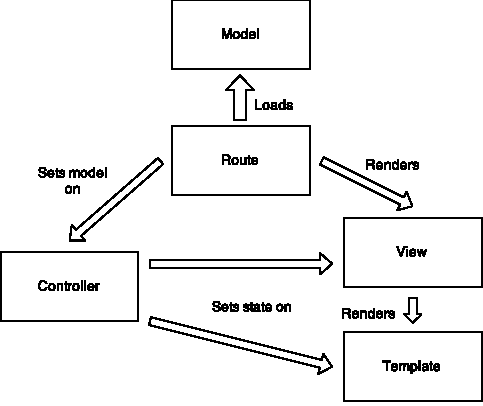
\includegraphics[width=10cm]{1_ember_architecture}
\caption{Ember framework architecture}\label{ember_architecture}
\end{figure}

Until now everything discussed was related to building the front part of a modern web application. But a web application consist also from the backed part. The HTTP application which listens client requests. For building one there are a lot of frameworks which easily allows to scaffold a prototype. MVC based frameworks are powerful and provides lots of functionalities out of the box. And the good thing is that the majority of frameworks are mature and stable. Here are a list of frequently used solutions:
\begin{itemize}
    \item Ruby on Rails
    \item Django
    \item Spring
    \item Symphony
    \item ASP .NET
\end{itemize}
The thing is that the mentioned technologies have huge stacks which sometimes are not needed when building a smaller application, or scalable one. Besides for building modern web applications where the client application is developed in a Java Script framework, means that the "V" (view) part from MVC is not needed anymore. Plus there are already on the market lightweight web technologies such as Sinatra, Flask, Node (in combination with express library). This type of application can serve just as good. In case if new module is required by the application, it can be easily added to the micro-framework stack. In ruby this is done by using gemfiles (gems are libraries in Ruby language) were gems can be easily added and installed effortlessly.

\subsubsection{Web Sockets}
\subsubsection{Data Visualization}
\subsubsection{HTML Parsing}
\subsubsection{Data storage}

\subsubsection{Data Journalism}
According to wikipedia, Data journalism is a journalism specialty reflecting the increased role that numerical data is used in the production and distribution of information in the digital era. It reflects the increased interaction between content producers (journalist) and several other fields such as design, computer science and statistics. From the point of view of journalists, it represents "an overlapping set of competencies drawn from disparate fields". \cite{wiki_data_journalism}

The journalists main resource for their work is data, and it was so from the very begging of the journalism. The computer revolution from the 20th century revealed massive opportunities for an a lot of economical fields (and not only). Journalism started integrating data by bringing computer technologies into their daily lives. The nowadays explosion of technologies such as Internet, cloud computing, high performance of mobile devices, easy accessible open source software influenced a lot the modern journalism leading to emergence of data journalism. This new term represents a new extended branch of traditional journalism by involving more data in the field. Decades after early pioneers successfully applied computer-assisted reporting and social science to investigative journalism, journalists are creating news apps and interactive features that help people understand data, explore it, and act upon the insights derived from it. New business models are emerging in which data is a raw material for profit, impact, and insight, co-created with an audience that was formerly reduced to passive consumption.

Journalists around the world now are faced with exciting challenges of writing reports and stories based on deductions made on vast amount of data which is daily increasing and changing. The data generation source are diverse, network lives, businesses, government, politicians, popularities etc. While the potential of data journalism is immense, the pitfalls and challenges to its adoption throughout the media are similarly significant. Global threats to press freedom, digital security, and limited access to data create difficult working conditions for journalists in many countries. A combination of peer-to-peer learning, mentorship, online training, open data initiatives, and new programs at journalism schools rising to the challenge, however, offer reasons to be optimistic about more journalists learning to treat data as a source.

Data visualization is an entire field which is developing alongside data growth. While the tools for visualization are interesting and fancy, visual results alone does not represent much value. It is the story and conclusions which can be drawn from the visual tools what actually matter. A good analogy is the bread preparation, the whole chain of events, starting from sowing the seeds and ending with backing the bread. The story represents the bread in this cycle, the final result, the product which can be published and consumed.The embrace of open source software and agile development practices, coupled with a growing open data movement, have breathed new life into traditional computer-assisted reporting. Collaboration across newsrooms and a focus on publishing data and code that show your work differentiate the best of today’s data journalism from the CAR of decades ago.

Data journalism can be created quickly or slowly, over weeks, months, or years. Either way, journalists still have to confirm their sources, whether they are people or data sets, and present them in context. Using data as a source would not eliminate the need for fact-checking, adding context, or reporting that confirms the ground truth. Just the opposite, in fact. Around the world, a growing number of data journalists are doing much more than publishing data visualizations or interactive maps. They are using these tools to find corruption and hold the powerful to account. The most talented members of this journalism are engaged in multiyear investigations that look for evidence that supports or disproves the most fundamental question journalists can ask: Why is something happening? What can data, related to narrative structure and expert human knowledge, tell about the way the world is changing?

In the hands of the most advanced practitioners, data journalism is a powerful tool that integrates computer science, statistics, and decades of learning from the social sciences in making sense of huge databases. At that level, data journalists write algorithms to look for trends and map the relationships of influence, power, or sources. As they find patterns in the data, journalists can compare the signals and trends they discover to the shoe-leather reporting and expert sources that investigative journalists have been using for many decades, adding critical thinking and context as they go. In addition to asking hard questions of people, journalists can now interrogate data as a source.

\subsubsection{Web services}
Building complex systems is not a simple task to do and usually they consist of smaller logical parts which communicates trough interfaces. A modern distributed application usually runs on different machines. This is a wise choice to do, for multiple reasons. One is the easiness to troubleshoot problems. But with great power comes great responsibilities. On one hand it might prove quite difficult and expensive to run instances of different applications to run the system, on the other hand it can scale efficiently with the increasing demand. One more case might be to build an application which integrates many other public available services and APIs. In the end the point is that the applications should be able to communicate efficiently over the web. Various software are built in different programming languages, are running on diverse operating systems, hence a transparent communication model is needed which is language agnostic. That is how the web services protocols came to existence. During the time they have evolved into a set of communication standards which offered developers the opportunity to construct decoupled systems. The more decoupled the application is, the more testable and maintainable it is.

In order to define the standards, a set of rules are needed to be defined, such as:
\begin{itemize}
    \item How can a software perform a request to another system
    \item What is the set of parameters should be set in the request
    \item What should be format of the request
    \item What are the logical parts from which the request consists
    \item How should the response be represented
    \item How should the errors be described
\end{itemize}

As a result, on the market persist two approaches of constructing web services, SOAP and REST. Each approach have their strong points and weaknesses and both heavily relies on HTTP protocol, in case of SOAP it also supports other transport protocols.

\paragraph{SOAP}
SOAP is a messaging protocol which have the entire architecture wrapped around XML data representation. In a nutshell, it is a method of communication between two applications. An example of SOAP communication is represented in figure \ref{soap} The protocol specifies how exactly the HTTP headers should be encoded. A SOAP provider comes in hand with a WSDL file which represents the description of the web service. Things like the possible parameters and their formats, the structure of the message, what is the response format, how it can be correctly accessed. The communication via SOAP protocol is also done using an XML formated files. The structure of the the request and response is documented in the WSDL file and it is validated with the help of XSD schema.

\begin{figure}[!ht]
\centering
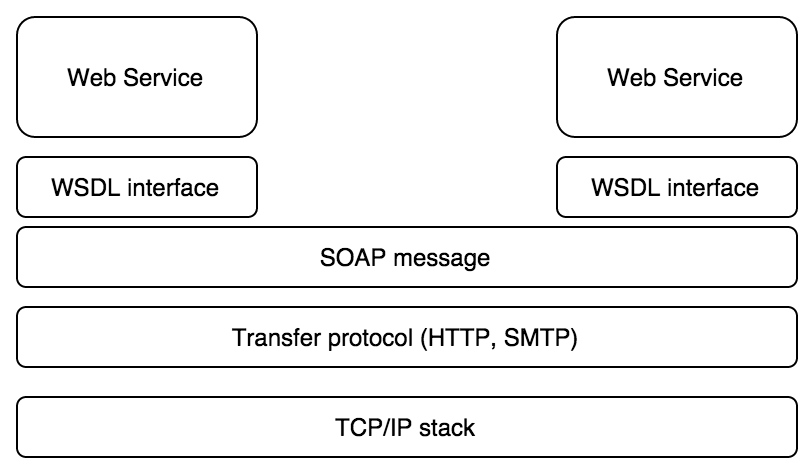
\includegraphics[width=13cm]{1_soap}
\caption{An example of SOAP communication}\label{soap}
\end{figure}


SOAP represents the next evolving stage between computer communication at he application layer. It was able to replace RPC technologies such as DCOM, CORBA, Java RMI. This reinstatement was highly needed because RPC technologies were brining a complex coupling to the programming language, which might prove a bad thing, as long as a panacea type programming language does not exist. On the other hand the SOAP calls are much slower comparing to native RPC applications. There tends to be firewall latency due to the fact that the firewall is analyzing the HTTP transport. SOAP calls are much more likely to get through firewall servers, since HTTP is typically Port 80 compliant, where other calls may be blocked for security reasons. Since HTTP requests are usually allowed through firewalls, programs using SOAP to communicate can be sure that the program can communicate with programs anywhere. SOAP is focuses on exposing pieces of application logic (not data) as services, platform operations. It aims for accessing named operations, each implement some business logic through different interfaces. An advantage offered by SOAP is the WS-Security which adds some enterprise security features. Supports identity through intermediaries, not just point to point (SSL). It also provides a standard implementation of data integrity and data privacy.

\paragraph{REST}
REST is a simple stateless architecture that generally runs over HTTPS/TLS.
This type of web service focuses on a reduced and very well defined amount of operations. The most common operations provided by a REST platform are CRUD. 
The flexibility is given by assigning resources their URI. The neat part is that it heavily relies on URLs. The REST philosophy is deeply entangled with HTTP protocol implementation, for instance the HTTP verbs GET, POST, PUT, DELETE, PATCH etc, are a part of REST RFC. Although it is just a set of guidelines and best practice, if implemented correctly the application avoids ambiguity. This is a blessing and a curse at the same time. Due to the fact that REST RFC is not a set of rigid requirement, developers tend to misinterpret the usage of some methods method. And example is overusing the "POST" method. Hence a lot of debates, discussions and even holly wars are held on this topic. The good part is that it doesn't need tedious descriptor files such as WSDL in order to describe a REST application. The documentation is usually done in textual manner, just like code documentation. REST gained a lot of popularity as being a simpler alternative to SOAP and WSDL-based web services. And the most viable example is the implementation of the entire Word Wide Web. One strong thing wielded by REST applications is that the message and response content can be delivered in any type of format. The most used are XML based format such as HTML, and for API platforms JSON is the most common and handy format, and it has lots of advantages against XML, such as readability, payload size, easy integrable with dynamic languages, it is data oriented.

Nowadays JSON is becoming the preferred format especially for RESTful APIs. Because of the format simplicity sometimes it gets harder to define the communication structure. Which is why JSON community is working now on an elegant format called JSON-api. It simplifies a lot things in terms of message structure. It resembles to WSDL only it is less restrictive and more intuitive. Another alternative for structuring the message format is HATEOAS. The purpose it aims is defining application state using hypertext.

\subsubsection{Hadoop Mapreduce}
In the last 10 years terms like Big Data, NoSQL, Hadoop, Mapreduce were so frequently discussed that some of them became bloated. For instance, what is Big Data? how "Big" is the data? In 2003 Google released a paper about Google File System, and later in 2004 a Mapreduce paper. Being a company which works with indeed extremely big data, sizes in terms of petabytes and more, they have started to search for solutions how to manage such amounts. And due to the fact that the computational power was getting cheaper by day, they have come up the idea of building file systems which would be able to run on computer clusters. In the path of finding the methods to operate with the huge amounts of data they have seen that the traditional RDBMS database engines would not fit their requirements, so they've came up with an alternative. On 2004 they started working on a new kind of data base based on a different concept, BigTable. A database which exchanges the classical ACID rules with scalability, availability and other positive aspects which would solve their problem. Of course Google is not the only company working with huge amounts of data, resulting in other technologies which were developed based on similar concepts. For instance Amazon came up with DynamoDB, a database which works on the same principle as BigTable, instead it was focused on offering availability instead of consistency (a customer should always be able to buy even though the product is not present in stock). Another example is Yahoo, who came up with Apache Hadoop, a great technology released under the Apache open source license. It is a files system which can work on multiple computers and indeed successfully solve the problem of processing big amounts of data.

After the successful stories of the leading companies, the terms Hadoop, BigData, NoSQl, started to become popular and spread like a fever. Of course lots of companies started using this technologies, because you have to follow the cool kids. The problem was that companies, especially new one, were not making the business smart decisions when choosing the technologies. For instance building an application using a schemaless database. After making the wrong decision it was realized that the application structure actually needed schema. It resulted in managing schema consistency by the application layer, which is an additional layer of complexity that can be handled by a traditional RDBMS engine. A analogous story is related by the Olery company \cite{mongo_to_postgres}. Many startups started to use the newly discussed solutions, forming communities, thus the deceiving labeling started. Everything which is not RDBMS is NoSQL, a term which was intended to be used as a twitter hashtag now covers under it's umbrella all the databases which does not rely solely on ACID principles. The same situation is with Big Data. What is the actual size of the data required for being called "big". There are lots of speculations on this topic.

\paragraph{Hadoop}
Hadoop is a framework used for distributed storage and distributed processing of large scale of data sets. It can benefit from cheap computation power by running on a mediocre computer cluster. The platform is designed by taking into consideration the hardware failure. It is natural that at some point in time a machine from the cluster will stop running. Hadoop embraced this problem and solved it at the software level. Although Hadoop is best known for MapReduce and its distributed filesystem (HDFS, renamed from NDFS), the term is also used for a family of related projects that fall under the umbrella of infrastructure for distributed computing and large-scale data processing. As the Hadoop ecosystem grows, more projects are appearing, not necessarily hosted at Apache, which provide complementary services to Hadoop, or build on the core to add higher-level abstractions.

Applications that run on HDFS have large data sets. A typical file in HDFS is gigabytes to terabytes in size. Thus, HDFS is tuned to support large files. It should provide high aggregate data bandwidth and scale to hundreds of nodes in a single cluster. It should support tens of millions of files in a single instance.

HDFS has a master/slave architecture. An HDFS cluster consists of a single NameNode, a master server that manages the file system namespace and regulates access to files by clients. In addition, there are a number of DataNodes, usually one per node in the cluster, which manage storage attached to the nodes that they run on. HDFS exposes a file system namespace and allows user data to be stored in files. Internally, a file is split into one or more blocks and these blocks are stored in a set of DataNodes. The NameNode executes file system namespace operations like opening, closing, and renaming files and directories. It also determines the mapping of blocks to DataNodes. The DataNodes are responsible for serving read and write requests from the file system’s clients. The DataNodes also perform block creation, deletion, and replication upon instruction from the NameNode. In figure \ref{hadoop_architecture} is represented the HDFS architecture.

\begin{figure}[!ht]
\centering
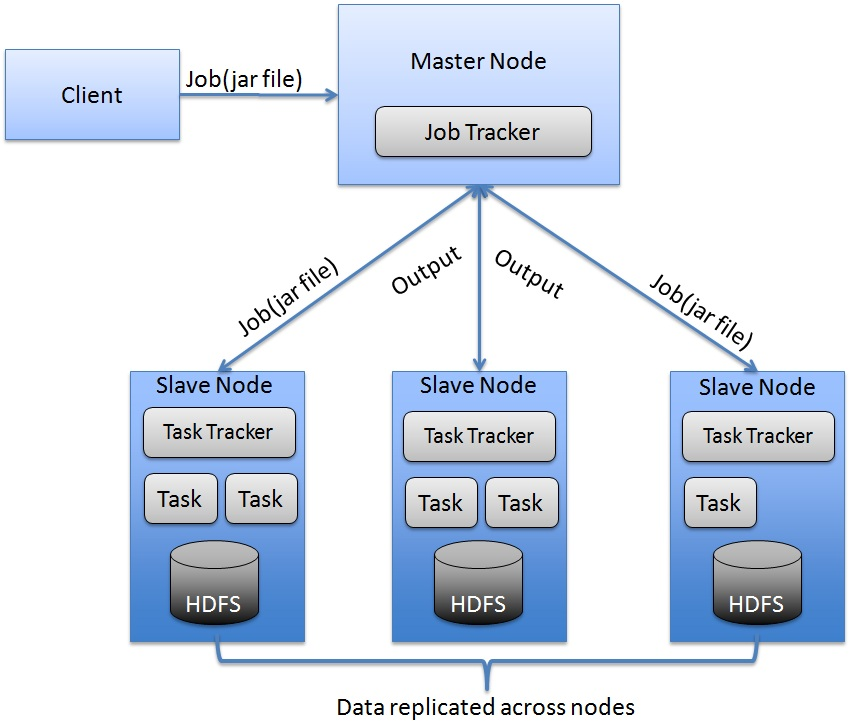
\includegraphics[width=13cm]{1_hadoop_architecture}
\caption{Hadoop architecture}\label{hadoop_architecture}
\end{figure}

The NameNode and DataNode are pieces of software designed to run on commodity machines. These machines typically run a GNU/Linux operating system (OS). HDFS is built using the Java language; any machine that supports Java can run the NameNode or the DataNode software. Usage of the highly portable Java language means that HDFS can be deployed on a wide range of machines. A typical deployment has a dedicated machine that runs only the NameNode software. Each of the other machines in the cluster runs one instance of the DataNode software. The architecture does not preclude running multiple DataNodes on the same machine but in a real deployment that is rarely the case.

\paragraph{Mapreduce}
The conceptual logic of Mapreduce is a primitive one. The approach it has looks like a brute-force. It is a batch query processor, and the ability to run a query against an entire dataset and get a result in reasonable amount of time is an astonishing thing. It opens an entire new perspective of processing data. The algorithm works in the following way. The user specify a map function which is applied to every record. The goal is to emit a key value pair to generate a set of intermediate key/value pares. The reduce function merges all intermediate values associated with the same intermediate key. Many real problems can be modeled under this concept. Programs written in this functional style are automatically parallelized and executed on a large cluster of commodity machines. The run-time system takes care of the details of partitioning the input data, scheduling the program’s execution across a set of machines, handling machine failures, and managing the required inter-machine communication. This allows programmers without any experience with parallel and distributed systems to easily utilize the resources of a large distributed system. Here is an example of map reduce executed in MongoDB \ref{mongo_example}. MongoDB api involves a native Mapreduce feature.

\lstinputlisting[language=Python, caption={Mapreduce example in MongoDB}, label=mongo_example]{../src/map_reduce_example.js}

\subsubsection{Lexical analysis}
Open Media project works with articles fetched from the available public sources. As data value it represent just massive chunks of text. Working with plain text might prove a problematic. The reasons are that a spoken language such as English or Romanian (in this particular case) are vast and complex. More than that they might prove to be ambiguous. A simple task like determining the part of speech of a specific word might prove a complex action. The same word might have different meanings in different circumstances. Which is why a probabilist model based on machine learning has to be constructed in order to detect word's context and determine the part of speech it belongs to. Having a text enriched with metadata such as a part of speech is proved to be useful for advanced text analysis. A trivial case is for eliminating the stop words. There are different approaches for this problem. First one is having a dictionary with stop words and check every word if it is a part of the record. The second approach is to assume that all the stop words have a length lesser than for. The issue with this is that there are a lot of exception thus not feasible to fit cluster the words solely on number of characters. The approach which will have an acceptable error rate and will work quite fast (in comparison with a dictionary check) would be, first to detect the part of speech, followed by words elimination which refers to the stop word part of speech.

The process described above is one of the many kinds of text preprocessing tasks which involves lexical analysis. Many of theses processes work hand in hand with another. Usually one can operate on a dataset which is a result of the previous one. Here are listed one of the operations regarding lexical analysis:
\begin{itemize}
    \item Tokenization
    \item Part of speech tagging
    \item Lemmatisation
    \item Text Segmentation
    \item Chunker
    \item Syllabification
    \item Stemming
\end{itemize}

\paragraph{Natural Language Processing}
Almost all the mentioned above operations are a result of NLP area. It is a field of computer science, artificial intelligence and computational linguistics which studies the interactions between computers and human languages. One of the main challenge of this field involves natural language understanding, where computers are able to extract meaning out of human language input. The classic approach of solving this problem was by hand coding a big set of rules which the machine has to follow. In such way decision trees models were created, basically a lots of "if else" statements. But unfortunately a natural language is a rather complex concepts, and catching all ambiguities makes the decision tree unmaintainable. In the end the traditional decision trees usually resulted in a rather primitive solution. Modern NLP uses lots of machine learning algorithms under the hood. The idea is to apply the learning on a set of corpora where a corpus is a set of documents, sentences which have been hand-annotated with the correct values to be learned. The annotations representing metadata such as part of speech, the word root, synonyms etc. Having a probabilistic model gives the advantage that in a specific situation the solutions can be multiples, with different chances. Usually such type of results are better suited as being a part from a larger system.

\paragraph{Tokenization}
NLP field requires at beginning much primitive actions. The first being the tokenization. It represents the process of breaking a string into words, symbols, phrases or other meaningful elements which could be called tokens. Typically the segmentation is done at the word level. The traditional implementation relies on simple heuristics. Tokens are usually separated by whitespace or punctuation characters. Most of Latin alphabet based languages use inter-word spaces (eg New York-based). For such kind of languages the solutions is straightforward. The grade of complexity is much more increased for languages written in scriptio continua such as Ancient Greek, Chinese, Thai.

\paragraph{Lemmatization}
Another important part of text analysis is lemmatization. The idea behind it is to reduce the word to a canonical form. Similar words, or with the same root would have the same result after passing the lemmatisation process. This will give the opportunity to operate with a group of words from the perspective of a single entity. The stemming process is rather similar. The difference is that stemming can be applied to an independent word, while lemmatization works based on the word context, meaning that it has a more complex algorithm on the background. The process already requires additional metadata such as the part of speech of the word. Even though the stemming algorithm is more primitive, due to the fact that it doesn't discriminate the word meaning, the implementation algorithm is much simpler. This fact gives an upper hand for a data analysis process, especially when the computational speed is the bottleneck. An example of lemmatization is that the algorithm ensures that "traveling", "traveled" will be recognized as the same word "travel". This aspect is crucial in context of OpenMedia, if the words are not brought to a canonical form, then the frequency analysis would have an increased error rate, which would lead to an unreliable platform not likely to be used by users.

\subsubsection{Data Mining}
According to wikipedia sources, data mining, an interdisciplinary subfield of computer science, is the computational process of discovering patterns in large data sets involving methods at the intersection of artificial intelligence, machine learning, statistics, and database systems. The overall goal of the data mining process is to extract information from a data set and transform it into an understandable structure for further use. \cite{wiki_data_mining}

\begin{figure}[!ht]
\centering

\includegraphics[width=9cm]{1_data_mining}
\caption{Data Mining}\label{data_mining}
\end{figure}

The purpose of data mining is to conduct automatic or semi-automatic inquiries on large amounts of data in order to extract patterns such as groups of records, unusual data, dependencies. In order to perform operations of this scale usually special database techniques are needed. One of are them spacial indexes. This kind of indexed is created based on geospatial data structure, and it helps to increase the performance for queries such as finding the distance between two places. The kinds of patterns detected in a data mining task can be use for further analysis, machine learning, events prediction. Twitter introduced a curious research, based solely on people tweets they have created an influenza pandemic prediction model. It is astonishing that a platform used for posting short textual messages was used for predicting a biological phenomenon. What if the research is done on a dataset strictly target to the analyzed field. Another successful data mining research was done for exploring some specific cancer drugs. Before the research, the result was that the drug (eg X) was working in the 20\% of cases. After the genetic research, it was found out the patient's genetic configuration of successful cases. Now it was possible to identify the people to whom the drug X will work for 100\%. The examples described above tells how useful data mining could be and how wide is it applicable.

Data mining is not a solitary field. It takes advantages of more mature fields such as artificial intelligence and statistics. All these fields work hand in hand on problems such as pattern recognition and classification. Both fields have researched the understanding and applicability of neural nets and decision trees. To make it more clear, data mining it's not an autonomous approach of solving this problems but more like an enhancement of traditional statistical models. The development of traditional statistical techniques was done based on elegant, mathematical based, theories that worked fine on small amounts of data. The problem that the amount of generated data per day is increasingly drastically, mainly because the source are mostly machines. Log files, sensor output, data generated by other data generated by computers. And when it comes to analyzing it, the classical models will not apply. The need to analyze enormous data sets coupled with low cost computational power, allowed the development of new techniques based on brute-force exploration of possible present solutions.

Data mining is started to become more and more popular because of the substantial contribution it can bake. It can be applied to control product costs or to increase the revenue. Popular organizations use data mining for managing all phases of the customer life cycle such as attracting new customers, increase sales from current customers, retaining good customers etc.
By profiling the preferences of good customers the organization can target customers with the same characteristics. Or by having gathered the information about the customers that left, it can be deduced on what points to focus in order to keep the customers longer in the system. Data mining offers value across a broad spectrum of industries. The main industries which profits from data mining techniques are credit card companies and Telecommunications. Insurance companies and stock exchanges apply this technology to reduce the fraud. Companies active in the financial markets use data mining to determine market and industry characteristics as well as to predicting individual company and stock performance. Retailers are making use of data mining by analyzing the bills and find which products occur more frequently together. Using this kind of information they rearrange the product positions. Or ti can be used to compute the effectiveness of promotions and coupons, everything done for maximizing the cash flow. Data mining field is indeed a widely used field and proved to have outstanding results for the time being.

\subsubsection{Text processing}
The aim of text processing is to consume unstructured textual information, extract important numeric indices and make it accessible for various data mining, statistical algorithms. Information can be extracted to derive summaries for the words contained in the documents or to compute summaries for the documents based on the words contained in them. Hence a text analysis can be performed on clusters of words used in documents. Another approach could be to analyze documents and determine similarities between them or how they are related to other variables of interest. In a nutshell, text processing is an action of transforming text into numbers, and other metadata, eventually used in predictive data mining projects, machine learning, data warehousing, etc.

Unstructured text is very common, and in fact may represent the majority of information available to a particular research or data mining project. A relevant example of textual data analysis application would be automatic filtering of undesirable junk emails based on certain terms and words that are most likely to be met. In such manner the obnoxious mails can be discarded. It can be taken even further, such kind of applications could be used in a bigger systems for routing messages, based on email contents, to the appropriate department. Or sent back to sender, in case of detecting some obscure content, with a request to change the body.

A powerful use case could be to process the contents of a particular Web portal. For example for extracting relevant specific block, and determining the most frequently mention word, thus deriving the most important terms of the web application. It's easy to observe how this kind analysis could deliver valuable business intelligence. This kind of use case resembles very much with system requirements of the OpenMedia platform. Given that the aim is to crawl all the possible articles of the media portals, and perform data mining algorithms on it. And as a result to have a set of services providing statistical .

Another curious aspect of data processing is that there are two angles of processing textual documents. First is many data to few documents, and second is small data from lots of documents. For instance, on case is performing complex text analysis tasks on few lengthy resources (like books) and the another is extracting key values concepts from tweeter messages which have a limit size of 140 characters. The second case is more compliant to statistic algorithms by the fact that the amount of data sources is much bigger. This means that OpenMedia is a perfect playground for applying various statistic models.

One think that should be taken into consideration is the data indexing. Indexing is a feature usually provided by the modern databases. The idea behind it is to create additional data, resembling a hash map data structure, which allows to search data much faster by a specific field. For instance we have classic SQL database with a "user" schema which has "name" field. If the system using the database is frequently searching for "user" entity by it's "name" then it is the most wise to perform indexing on the table. This will add additional data on the disk, instead the search queries by "name" would be much faster. The point is when dealing with big chunks of textual data indexing by each word my not prove a sensible option. Instead some tricks can be applied, like removing certain characters, words bounded by some length, frequently used stop words like "the", "a", "of" etc. Another idea would be a custom indexing task which would detect synonyms and index as the same entity when a pair is found. One more thing would be to remove the rarely used words which do not offer much information about the text.

\subsubsection{Web Crawling}
In context of OpenMedia, fetching the data is the first step in the system. And considering that the primary sources of raw data are the online public media, it would be a wise move to invest time in researching the concept of web crawling, how can it be used. What are are is crawler's architecture etc.

A web crawler (also known as a robot or a spider) is a system for downloading Web pages, usually in a batch manner. Web crawlers are used for a variety of
purposes. The most popular is being a part of a search engine. The main purpose is to fetch the pages, index it's content such that in result users could find it the page by querying the key words found on the page. A related use is web archiving, where large sets of web pages are periodically collected and archived for posterity. Another use (the one relevant to the project) is data mining, where web pages are analyzed for statistical properties, or where data analytics is performed on them.

Crawling is an action which can be performed from anywhere, could run on potentially hundreds of threads, each of which loops through the logical cycle. These threads may be run in a single process, or be partitioned amongst multiple processes running at different nodes of a distributed system. A crawler frontier is the stack of URLs from which is selected the next visited page. The crawling process start by taking a URL from frontier stack and starts fetching the web page at that URL, generally using the http protocol. The obtained result is saved into a temporary storage, a set of operations is performed on it, usually parsing the text, extracting new links to be added to the frontier. The text, with any tag information like terms in
boldface, is passed on to the indexer. For this purposes special tags and text enriching techniques are used to mark the important content on the web page. This is done solely with the purpose to make the web pages more likely be referred by the search engines. Next, a URL filter is used to determine whether the extracted URL should be excluded from the frontier based on one of several tests. For instance, the crawl may seek to exclude certain domains, for example .com  URLs, in this case the test would simply filter out the URL if it were from the .com domain. Web place certain portions of their websites off-limits to crawling, under a ROBOTS EXCLUSION standard known as the Robots Exclusion Protocol. This is done by placing protocol file with the name "robots.txt" at the root of the URL hierarchy at the site. The robots.txt file must be fetched from a website in order to test whether the URL under consideration passes the robot restrictions, and can therefore be added to the URL frontier. Due to the crawlers popularity, sitemaps protocol was adhered to the crawling concepts. It is an xml file which hints how it is better to crawl the specific web content provider. It includes the hierarchy of the web page, and metadata such as, what is the optimal frequency with which the page should be crawled. It is a handy tool because it meets the crawler halfway, and guides the optimal ways of extracting data.

The web crawlers are needed because the web is not information repository. It consist of millions of independent web content providers. Each one is providing their own service thus their own information structured as providers wants it. Web can be viewed as a agglomeration of content repository bounded together by a set of agreed-upon protocols and data representation formats. For instance Transmission Control Protocol, Domain Name Service, Hypertext Transfer Protocol etc.

In context of OpenMedia the crawling is planned to be done in an iterative way. Given that every article has an unique id by which it can be accessed, the only thing needed is to extract the latest article id (usually found on the main web page of the media portal). Having the latest article id, can be constructed the URLs for the all presumably existing articles and be pushed into crawler's frontier. This gives the means of collecting all the needed raw data.
\clearpage
\cleardoublepage

%CAPITOLUL2
\section{Software Design}
\phantomsection


\clearpage
\cleardoublepage


%CAPITOLUL 3
\section{Implementation Part}
\phantomsection
In the previous chapters were discussed the concepts covered by OpenMedia project. The research of the ideas is crucial given that the applications aims a niche which is relatively new in the market, in Moldova it is not even present. To be sure that the platform development start from the right foot, a thorough architecture design, modeled in UML language, was provided in the previous chapter. What follows now is the description of the implementation part. An exhaustive description of every step will be given, including code snippets, which technologies are used and the reason of their choice.

It ought be mentioned that the whole project is mostly written in dynamic language Ruby. Which is why the libraries and frameworks used by OpenMedia are from Ruby world. The secondary language is JavaScript. It is used for building the user interface and for some back end development mostly related to data preprocessing.

\subsection{Obtaining data}
Getting the raw data is the first part in the project cycle. The sources for extracting data are the public channels of media providers from Republic of Moldova. More specific these are Unimedia and Timpul. In further development more sources will be integrated in the system. Extracting each available article is not straightforward task. There are at least two approaches for solving this problem. First one involves social interaction, by contacting media representatives and asking access to the data they dispose of. The second way is to extract the data from the web sites hosted by media providers. Of course the second way is more tricky but at least it avoids the hassle with human interaction and also gives the opportunity to engineer the solution from a developer perspective.

In order to be able to get the data from the web sites one thing ought be clear. Every available article has a unique URL. Once there is a way to get the URL then getting the information is not a problem anymore. The classic way of collecting the URLs from a web page is to launch a crawler. Of course the web spider needs to be trained under the site specifications. This approach is usually chosen by the search engine. Their goal is to extract all the possible content and index the relevant data. The thing is that OpenMedia targets only the pages where only the articles are present. Given that articles from a single source has a unique template not prone to changes, the assumption that the URL also follows a specific pattern might prove useful. After some time and research it was observed that both Unimedia and Timpul article URLs have a similar pattern. Beyond that, in both cases were found unique identifiers in form of a number, for example an article from Unimedia looks like this \emph{http://unimedia.info/stiri/-94630.html}. The natural assumption is that in order to get the URLs for the remaining articles the only thing needed is to decrement the number in the URL string mentioned above. For Timpul media source the process is analogically. One important thing is to know the id range which articles can have. For solving this problem the identifier for the most recent article is extracted from URL. Once this information is available all the articles can be accessed in a simple and iterative manner. And no need for web spiders frameworks are required anymore.

Now that the logical flow of extracting article URLs is present, there are also other requirements like getting the page, saving it to file storage, archiving it first in order to diminish the content size. Also the manner of extracting the articles differ from one source to another. Which means that a custom script should be designed for every particular media source. Nevertheless it is a smart engineering decision to unite the scripts under the same interface. In the following snippet, listing \ref{unimedia_fetchre}, is represented the class used for extracting all articles from Unimedia source. It is an autonomous class with idempotent properties. Every time it runs it checks what is the latest article identifier, what is the most recently saved article and only after that it fetches the missing articles. For extracting web page content the application relies on rest client library \cite{rest_client_ruby}. This library is used in two cases. The first one is for extracting the latest article identifier and the second use case is for fetching article pages themselves. The fact that fetching data is a simple console application does not mean that it shouldn't have a user interface. In order inform the user about the fetching state, a console interface progress bar is used. It provides useful information like how many articles have been fetched, how many remains, what is the estimated time of processing. An example is given in figure \ref{fetcher_progress_bar}.

\begin{figure}[!ht]
\centering

\includegraphics[width=18cm]{3_fetcher_progress_bar}
\caption{Fetcher progress bar}\label{fetcher_progress_bar}
\end{figure}

After fetching the article it is archived and saved to file storage. The handy part of the current implementation is how easy is to integrate one more media source. The only thing needed is implementing a custom fetcher class that will follow the same protocols as FetcherPublica and will have implemented the "run" method. Another required change will be to add on more line of code in the script which controls the fetching process, listing \ref{fetcher_script}. Decoupling the logic offers an increased simplicity when a change in project is required. Following the good practices always generate a good result especially when a project evolves in a changing environment.

\lstinputlisting[language=Ruby, caption={Unimedia fetcher}, label=unimedia_fetchre]{../src/unimedia_fetcher.rb}

\lstinputlisting[language=Ruby, caption={Fetcher script}, label=fetcher_script]{../src/fetcher_script.rb}

Another thing is should be considered is the time of execution. The program heavily relies on network connection given that all the data are available on web. It is also important not to abuse the media sources. In case of too many connections the web server can just block the IP which would lead to an unpleasant situation. The point is that it is not worth to make the script work fast. More than that, in case IP blocking it might even require micro-sleeps between the requests. With this in mind, the resource fetching logic was encapsulated in a separate class. The SmartFetcher class is clever enough to add sleeps before making a request in case that the web server does not respond appropriately. Also it outputs different notification messages in case of unsuccessful request. The good thing is that any fetcher class is encouraged to use the SmartFetcher therefore all the heavy lifting is shifted to an already working part of application. Here is a snippet how the smart fetcher handle errors, listing \ref{smart_fetcher}

\lstinputlisting[language=Ruby, caption={SmartFetcher handling errors}, label=smart_fetcher]{../src/smart_fetcher.rb}

After running the scripts the following was obtained:
\begin{center}
 \begin{tabular}{|c c c |}
 \hline
 Source & Execution time & Storage size \\ [0.5ex] 
 \hline
 Unimedia & 75h & 1.64 GB \\
 \hline
 Timpul & 53h & 1.71 GB \\
 \hline
\end{tabular}
\end{center}

\subsection{Storing data}
Correctly storing data and choosing the right database engine is a tough decision. The problem grows even bigger given the various number of choices available on the market. That is why a lot of factors should be consider. How data would look like. Will it have a lot of relations. What is the estimate number of requests per a period of time. Will it scale in case of a spike of requests. How crucial is to keep the data consistent. Will the business logic imply a lot of updates upon the data. Will data follow a certain schema. What kind of operations are usually applied to data. These are one of the few questions which influence the decision of the database selection.

For OpenMedia project MongoDB was chosen \cite{mongodb}. It is a cross-platform document-oriented database. Being labeled as a NoSQL database it exchanges the traditional table-based relations over JSON type documents with flexible structure. Due to this features it makes the data integration easy and fast in some specific use cases of an application. It makes embedded data very easy to manage. Also it doesn't leave back all the features offered by a traditional RDBMS. It has indexes which work as well as in relational databases. The indexing is happening at embedded field level..

The main reason for choosing this engine is because it is schema-less. Even though the final client part of the application will have a defined schema. MongoDB leverages the flexibility that it provides. Due to the fact that the platform is expected to change its structure and functionality it would be much easier to do so when data is managed by MongoDB. Another critical part is data preprocessing. The number of phases in which data might shape is hard to forecast. The entire system behaves very much like a live organism. In order to easily grasp and adapt under the new requirements MongoDB will offer means for easily prototyping the needed result.

Another important tool offered by MongoDB is the support for native MapReduce operations. OpenMedia relies heavily on this type of operations. MapReduce is fundamental in the data preprocessing part. There is no doubt that this part could be managed at the application level, but it makes more sens to use the tools which offers easy and elegant solutions to the problem.

The second step of the application is to extract the articles content from the HTML files stored on disk space and save to a database, more accurately to MongoDB. This results in writing a set of XML parsers which will be executed on the fetched data. The parsers should be adapted under the custom preferences of a specific media channel. As only two sources are targeted by OpenMedia results in two custom classes. The implementation concept is analogically the same as the fetching part of the system. A set of classes that follow the same protocol such that they can be easily managed. In listing \ref{timpul_parser} is represented the implementation of the most relevant methods of TimpulParsert class.

\lstinputlisting[language=Ruby, caption={TimpulParser parse and save methods}, label=timpul_parser]{../src/timpul_parser.rb}

The code represents the idea how a parser works. Nokogiri library was used for solving the specific problem of HTML parsing \cite{nokogiri_gem}. It is a easy to use library which is able to digest an XML input and return a set of nodes in form of ruby objects with enhanced functionality. In the end the consisted data is extracted in form of a plain Ruby hash and saved to database. Now the important part comes, the communication between the Ruby language and MongoDB. Naturally a ruby library is used for achieving the communication. In context of OpenMedia is specifically used Mongoid gem \cite{mongoid_gem}. An ORM is an API written in a specific language which offers a communication between a database and a programming language. It does more than that, it has the purpose to map the fields from a database to an class instance understood by the programming language. Thus making data accessing activity in a manner easily understood by the OOP language. A well implemented ORM comes hand in hand with a rich and powerful DSL. Of course not all the feature could be accessed through an intermediary DSL but at least it provides the most common operations. On the other hand when it comes to MongoDB, the native API is accessible in JavaScript. Which means that is realistic to create an ORM almost as powerful as the native API. Mongoid is a library which fulfills the necessity of the OpenMedia platform. It even allows injecting JavaScript code. In order to be able to operate with the database using Mongoid a set of classes, usually called models, needs to be define which comply a certain protocol. The class should included the Mongoid::Document interface and all the fields should be specified alongside with their type. An example of such a class is provided in the following listing \ref{mongoid_model}.

\lstinputlisting[language=Ruby, caption={ParsedPage Mongoid model}, label=mongoid_model]{../src/mongoid_model.rb}


\subsection{NLP processing}
The natural language processing is one of the most challenging part of the project. And there are few reasons which are backing up the problem. The major problem is that the data used in OpenMedia project is just text in Romanian language. There is nothing wrong with Romanian. The problem lies in the libraries available for use. In order to successfully implement a decent NLP library it requires a lot of tedious work. And it can only be done within a joint collaboration between a group of computer science engineers and experts in the specific language. A modern NLP library is built using probabilistic models and machine learning that requires a lot of data under a special format. The special format should be provided under the form of big chunks of text manually annotated with metadata such as the part of speech, what is the text token etc. The point is that creating such a library is a laborious process that usually involves specially trained stuff with a PhD degrees. Overall there are already available frameworks which does successfully does the text processing part. The tricky thing is that most of them are for English language. When it comes to Romanian the sources are very limited.

Luckily there are few universities from Romania which does research in this area and already have successfully implemented a set of libraries that can be used in context of OpenMedia. Currently there are two sources which are able to provide such a service. Both are doing so only in form of a online service over SOAP protocol. The first source is Universitatea "Alexandru Ioan Cuza" din Iași\cite{uaic}. The second source is Institutul de Cercetări pentru Inteligență Artificială "Mihai Drăgănescu", Academia Română\cite{racai}. In scope of the currently project was chosen the least source only because it was first found. No benchmarks were done over the sources, but as a future perspective there will be done a set of tests which will check which source is more reasonable to use. Or if it is possible to use both sources at the same time. Given that NLP is a costly and a long process it would be fair to divide the labor. It is rather unfortunate that neither sources does not provide the service under a form of library. There are more issues when it comes to using a SOAP service. The first one is latency, every service provided on the web is much slower in comparison to natively running a software. The second problem is the dependency. When an entire product relies on an external service, the entire infrastructure is very fragile. What if at some point in time the service will simply shutdown will this mean the end of product? And the last issue is the ethical part. To build a product that could possibly be sold on the market on top of sources provided by an university is not the correct business approach.

Coming back to the implementation part. The NLP operations were encapsulated in a separate class, RacaiBuilder. The operations represent nothing more but SOAP calls to one of the mentioned services. Under the class hood there's nothing more than an adapter to a external web services. For a successful implementation "savon" library was used \cite{savon_gem}. It is a ruby gem which encapsulates the hassle of operating with SOAP protocol by providing a simple and well documented API. THe class RacaiFetcher was constructed in form of a builder in order to give the developer the freedom to chose the order of operations. In the following  listing \ref{racai_builder} is represented some of the NLP methods and the client SOAP client management withing savon gem.

\lstinputlisting[language=Ruby, caption={ParsedPage Mongoid model}, label=racai_builder]{../src/racai_builder.rb}

So far so good. Now that there is class which is able to apply NLP actions upon an input is a great achievement in the project. What remains is to extract the parsed articles from MongoDB and run them through NLP class. Also the structure of the output result will be stored back into MongoDB under a different format. Most of the queries will be done by a specific word. Which suggests that it would be a better idea to store every word as a separate record. Of course every record will also contain additional metadata which will permit to extract the needed result for data visualization. As it was mentioned, using web service for a big amount of data takes a big amount of time. Parsing the and extracting articles to MongoDB resulted in 453 Mb of textual data. It is not a big amount overall, but from analysis perspective it will still require a long period of time to execute NLP operations, especially when used via a SOAP service. In the end the execution time on an average home PC took around 14 days. And it generated 9.2 GB of data.

\subsection{Preparing data for visualization}
The NLP operations were executed on the raw textual data. This brought data one step closer to the visualization part. To be more clear it only needs to undergo the data preprocessing phase in order to be ready for data visualization. Of course there was an initial attempt to skip this phase of the cycle. By having at disposal mapreduce tool offered by mongodb it was easy to prototype how user requests would look like under a format of a mapreduce. In listing \ref{long_map_reduce} is represented the source code of such a task.

\lstinputlisting[language=Java, caption={User mapreduce request on unprocessed data}, label=long_map_reduce]{../src/long_map_reduce.js}

The execution time of the code shown above on an average PC takes around 5 minutes. The result is understandable considering that the dataset is around 10 GB. Still, it is a very long time for a single user request. The immediate feedback is crucial feature within a client based application. The bottleneck proves to be the large dataset. This means that data should go through a compression process but at the same time remain consistent. The NLP step generated a dataset in a format of every word in every article with metadata such as article\_id, published time, part of speech and the source. What user requires is the number of mentions per month and the media source of a specified word. In order to meet the user requirements the data can be stored in form of  {word, mentions, year, month, source}. In listing \ref{bend_map_reduce} is represented a mapreduce task which bends the data under the user requirements.

\lstinputlisting[language=Java, caption={Mapreduce job for data compression}, label=bend_map_reduce]{../src/bend_map_reduce.js}

It looks quite similar to the previous mapreduce. The only different thing is that it runs once there are data updates but not at every user requests. The resulted data size is 456 MB. This is a number that can be worked with. More than that, it has such a structure that the user requests no longer need to execute mapreduce tasks. It is just a simple query with a simple conditional which takes around 0.5 seconds. As it was mentioned before that MongoDB offers indexing features. After composing and index by the word field the query result improved even better. It got to immediate responses around few milliseconds. Data preprocessing is indeed an astonishing improvement to the system. It decreased the request time from five minutes to few milliseconds. Alongside the data compression mapreduce job another compression task is required. The job is intended to computes the number of published articles for every month for every media channel. This data is used to compute the a specific ratio. The number of articles which have the mentioned the word over the number of published articles in a single month.

\subsection{Visualizing the data}
Data visualization is the part that matters to the end user. Everything done until now does not have a value if data is not represented under a human readable format. It is important that data should be represented in such way that it would communicate a message. A message that is clear enough and from which viable conclusions can be drawn. In context of OpenMedia the only method for displaying data is the line chart. For every user requests there are available only two line charts. Even though it might be not very much, building the whole infrastructure took a lot of time and research. Besides in case there is a sudden idea to add a new type of search, or a new type of data visualization the implementation phase would be very easy due to the fact that there is a platform which backs up and does a lot of hard work regarding data flow.

The data visualization happens in a browser page. This concludes that the tools for building plots are JavaScrpit based libraries. OpenMedia platform uses D3 library for constructing visual data representations \cite{d3}. D3, coming from Data-Driven Documents, is a library used for constructing dynamic and interactive data visualization in a web browser. It heavily relies on SVG, HTML5 and CSS standards. The most powerful point of this library is that it gives a great control over the final result. Embedded within an HTML webpage, the JavaScript D3.js library uses pre-built JavaScript functions to select elements, create SVG objects, style them, or add transitions, dynamic effects or tooltips to them. These objects can also be widely styled using CSS. Large datasets can be easily bound to SVG objects using simple D3.js functions to generate rich text/graphic charts and diagrams. The data can be in various formats, most commonly JSON, comma-separated values (CSV) or geoJSON, but, if required, JavaScript functions can be written to read other data formats.

As it was mentioned there are only two types of line plots for every user requests. The line-plots depicts how in how many articles the specified word was mentioned in a month. The first chart computes the word frequency in relation with the total amount of articles published by the source in that month. The second plot simply shows the number of mentions of the word. In order to browse the plot information in a easy manner it was enhanced with tooltip feature. When a plot is hovered it shows how many mentions are present and what is the date to which the the data relates. A representation of the result can be observed in figure \ref{frequency_plot} and figure \ref{mentions_plot}.

\begin{figure}[!ht]
\centering
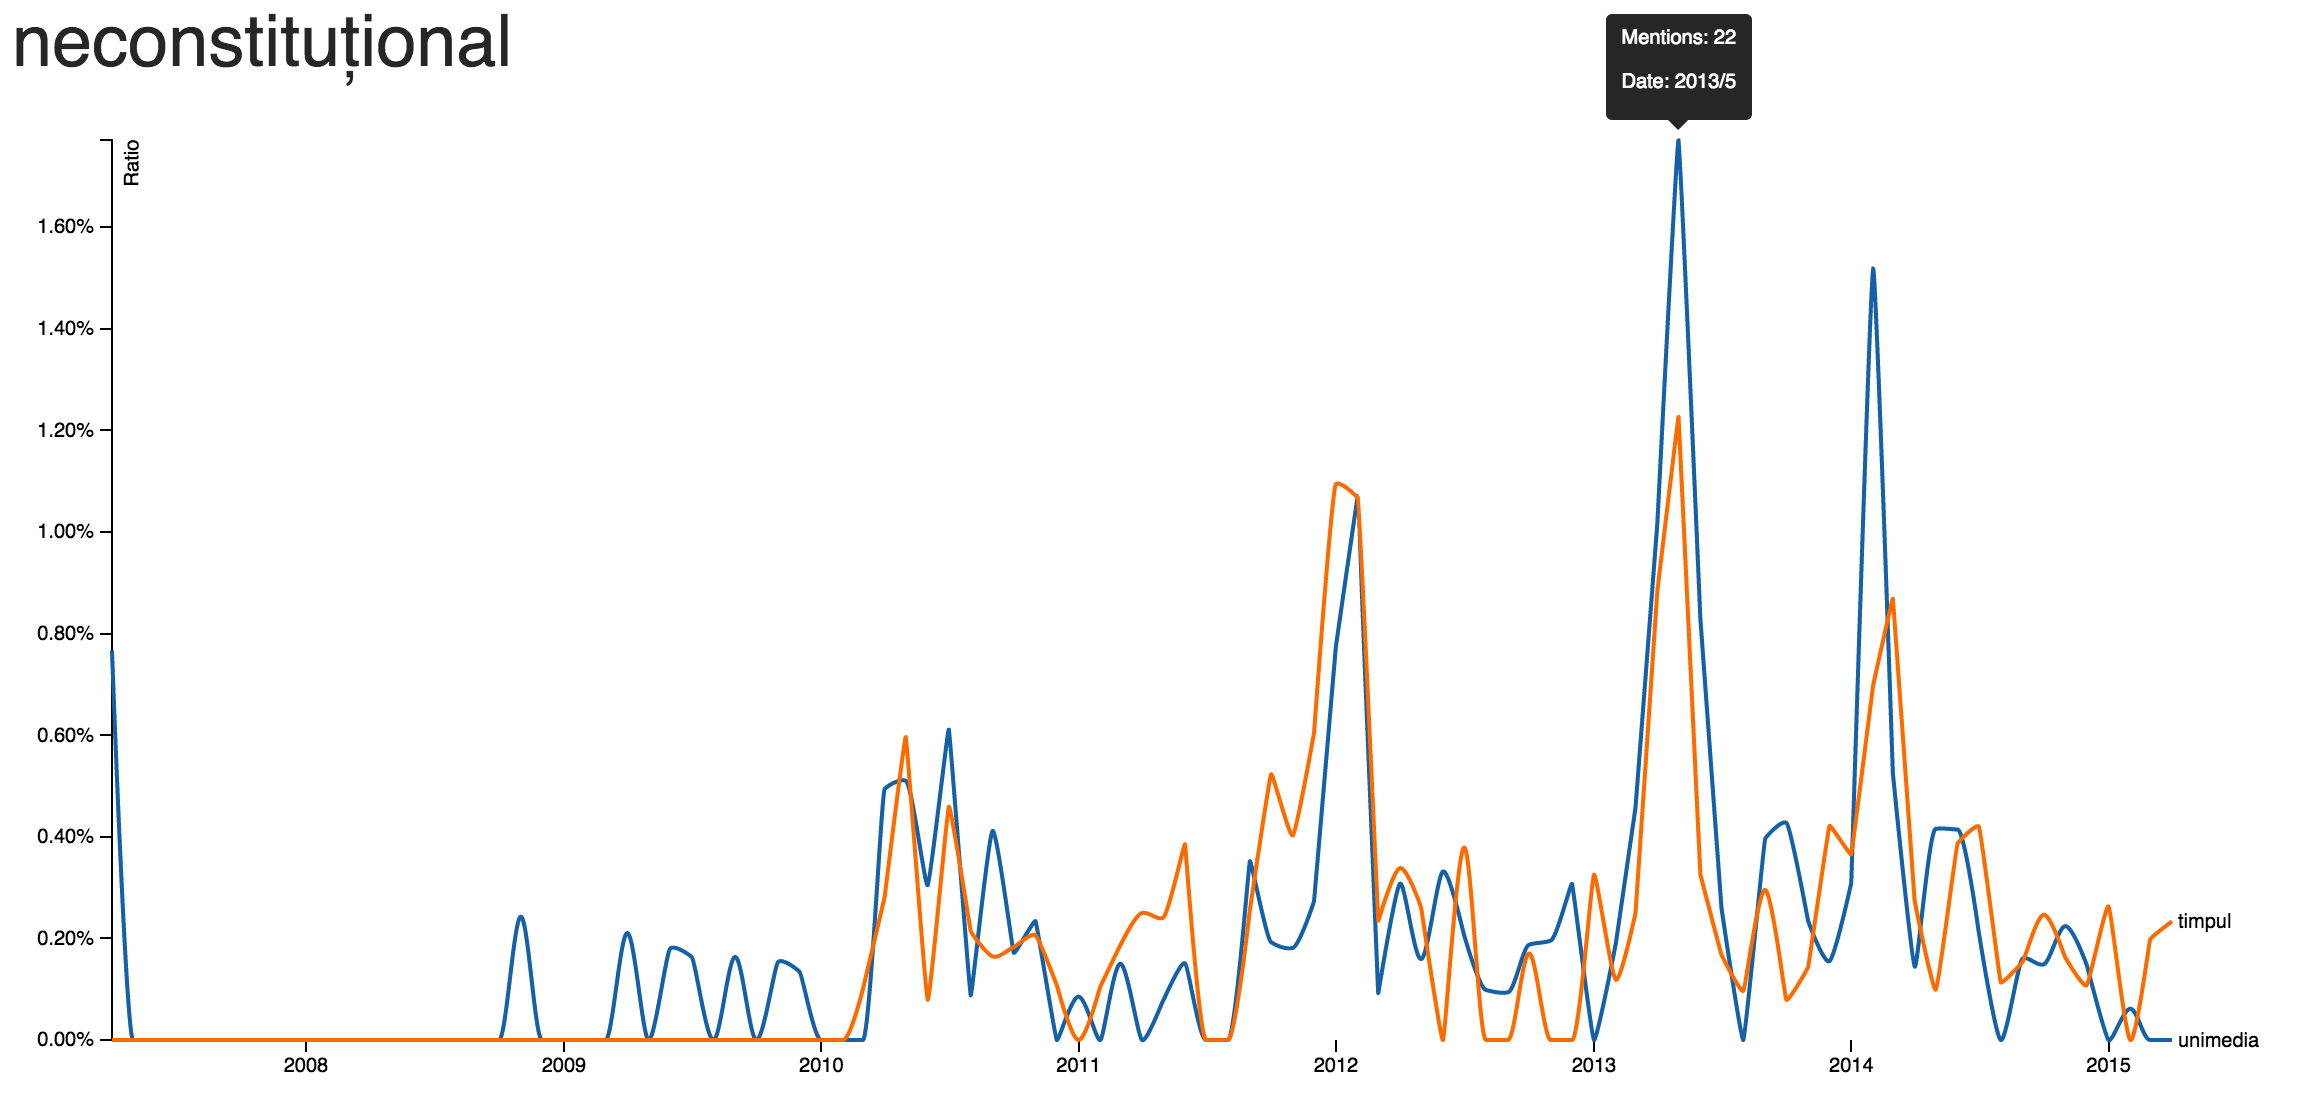
\includegraphics[width=15cm]{3_frequency_plot}
\caption{Frequency line plot}\label{frequency_plot}
\end{figure}

\begin{figure}[!ht]
\centering
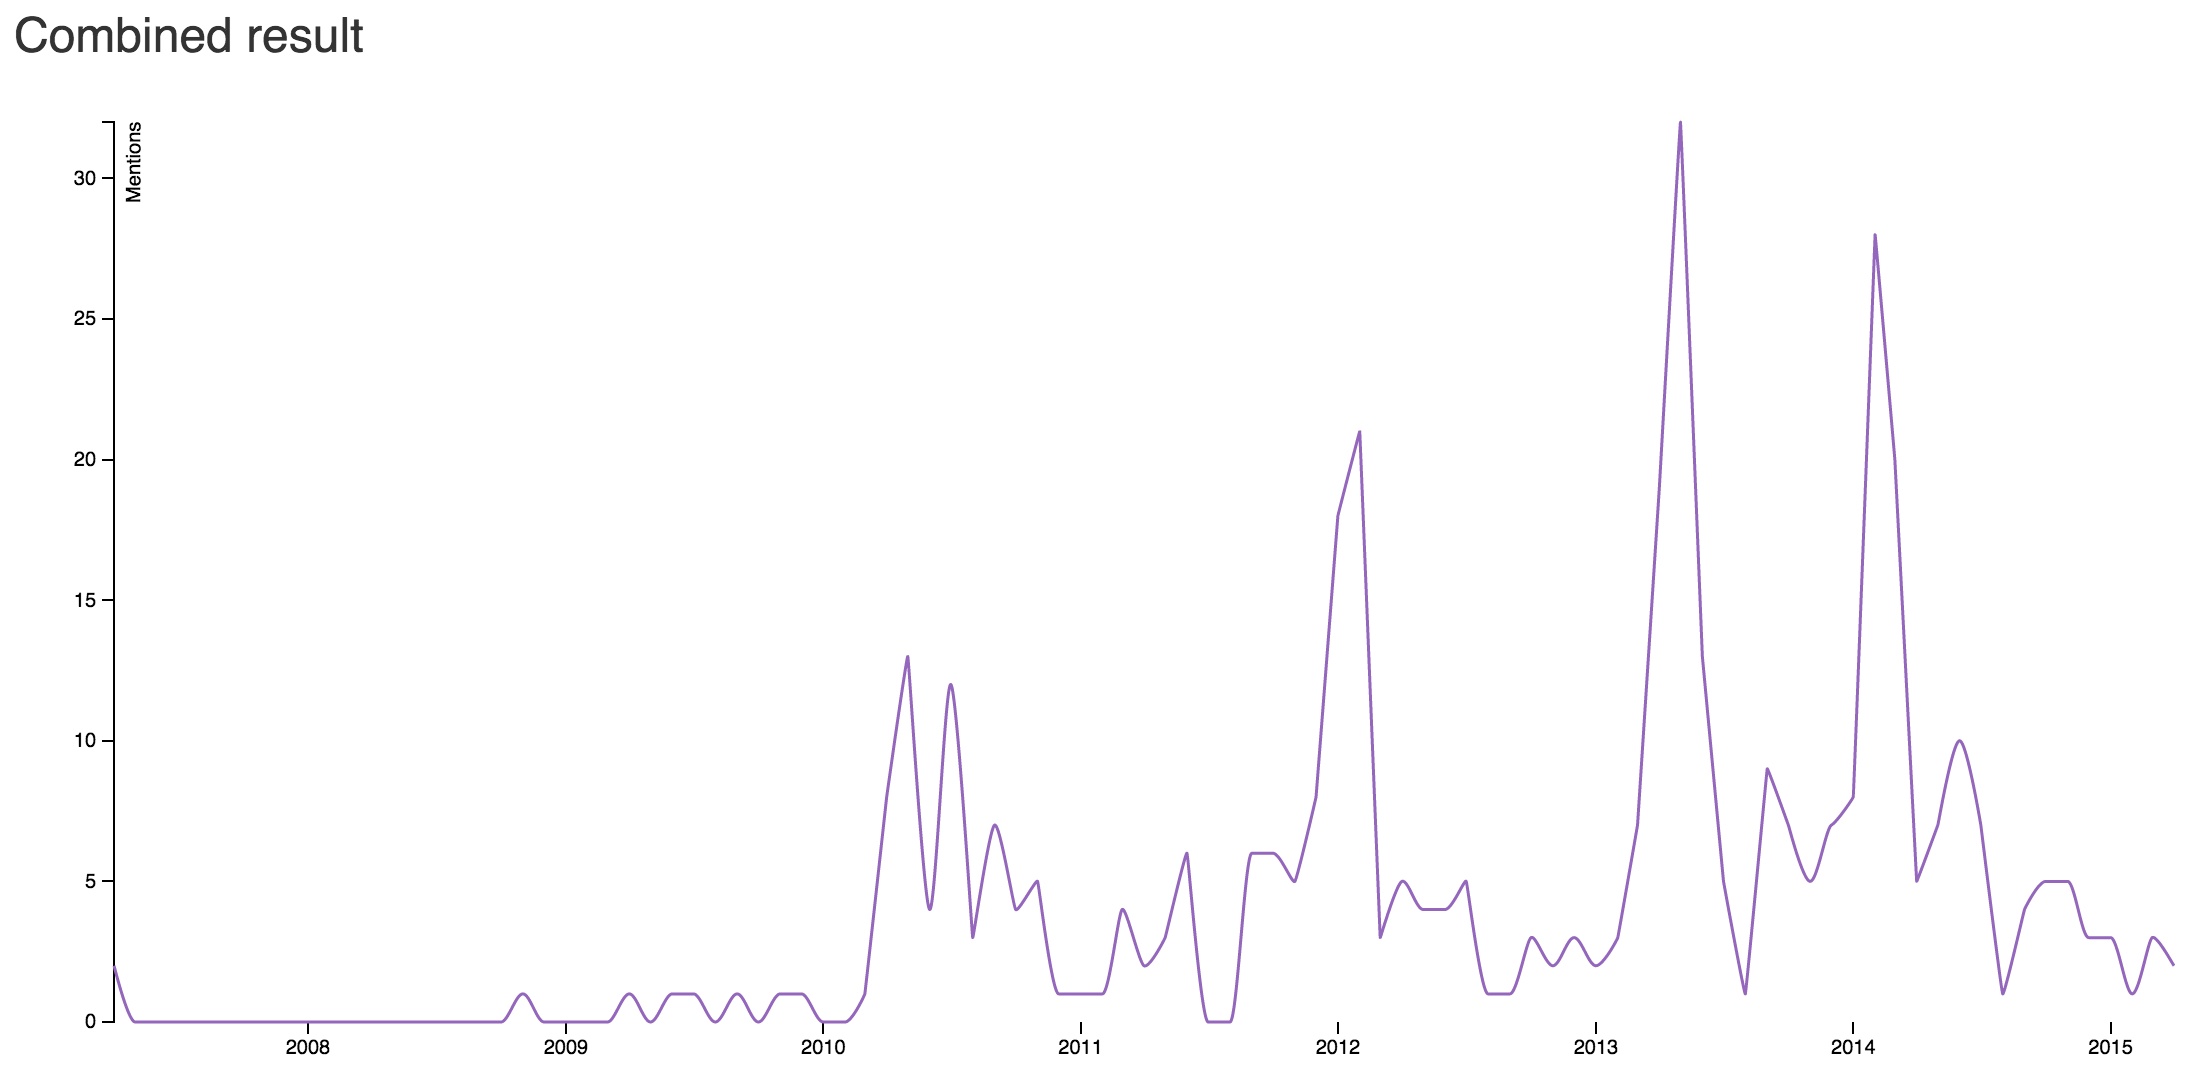
\includegraphics[width=15cm]{3_mentions_plot}
\caption{Mentions line plot}\label{mentions_plot}
\end{figure}
\subsection{Providing the UI}

\clearpage
\cleardoublepage

%CAPITOLUL 4
\section{Economic Analysis}\label{sec:economy}
\phantomsection

\subsection{Project description}
For the last decades the amount of generated data is raising exponentially. This phenomena is caused by the increased number of data sources provided by devices, sensors, log files etc. As a result there are tremendous amounts of data which can be explored and used for deducting useful information. There are various fields which profit from Big Data analysis, such as marketing, business, pharmaceutical, social science, fraud detection. Another interesting application of Data Mining is journalism. The combination of theses two caused the emergence of Data Journalism concept.

OpenMedia project is a platform for data journalism which is based on a wide range of available articles published using online sources. Data Journalism is widely used by the top newspapers reporters for deducing and writing a good article. Unfortunately data journalism is not practice in Republic of Moldova, thus it gives the project OpenMedia an upper hand by being first in this market. Also because the field is well explored by well developed countries, it provides a good source of examples. If a such a platform will exist on the local market, journalists would be able to write well documented articles on interesting and spicy topics. Hence offering a richer source of good articles to read. More than that OpenMedia provides a set of well defined visualization tools which can be used by business analysts, for better targeting the market and improving the CRM. From this perspective is it clear why a visualization tool is needed. It can be used by a wide range of people, but mostly targeting the journalist and business analysts.

Being a web application it will offer the flexibility of cross-platform advantages. Users from different fields would be able to construct their own statistical results for helping doing their job.

\subsection{Project time schedule}
For the accomplishment of a project it is necessary to establish a schedule. For the development of the OpenMedia application, agile project management is applied to offer flexible and iterative method of designing the application. It goes in 5 stages: planning, research, development, testing and deployment. The steps are repetitive and incremental.

\subsubsection{Objective determination}
The main objective of the following project is to provide a complete and functioning application for data journalism. Otherwise without a finished product there is no profit. More to that, it is important to market the application and get exposed to a large audience in need. This can be done by targeting first the journalism companies like Unimedea, Publika, JurnalTV. Another way is to market oneself on platform-specific stores. Since it is not a common piece of software, it creates a very specific audience of users. 

To keep up with the latest trends and researches, it is also an essential objective to keep updated and provide enhancements to the software. The lifecycle of the application will require bugfixes, interface changes, feature implementations. All of that will help the system still be trendy and up-to-date on the market.

\subsubsection{Time schedule establishment}
As it was said above the project will iterate over 5 steps: planning, research, development, testing and deployment. Naturally as most of the IT projects, it is subdivided into smaller parts. Planning step isn't supposed take up a lot of time, since the requirements are flexible. Moreover due to the research part the design solutions can change over time and open up new perspectives. The process of development is being split up in smaller tasks that can be accomplished within a 2-5 day period. Total duration of the project is computed using \eqref{eq:duration}.

\begin{equation} \label{eq:duration}
 D_T = D_F - D_S + T_R,
\end{equation}

\noindent
where $D_T$ is the duration, $D_F$ -- the finish date, $D_S$ -- the start date and $T_R$ -- reserve time. In table \ref{table:schedule} is presented the first iteration of the project schedule. It uses the following notations: PM -- project manager, SA -- system architect, SM -- sales manager, D -- developer.

\begin{table}[!ht]
\begin{center}
\caption{Time schedule}
\renewcommand{\arraystretch}{2}
\begin{tabular}{| c | >{\centering\arraybackslash}p{5cm} | >{\centering\arraybackslash}p{2cm} | c | >{\centering\arraybackslash}p{5cm} |}
\hline
\textbf{Nr} & \textbf{Activity Name} & \textbf{Duration (days)} & \textbf{People involved} & \textbf{Comments} \\
\hline
1 & Define the project concept and objectives & 5 & PM, SA, SM, D & It is a common task \\
\hline
2 & Perform market analysis & 10 & PM, SA & Will results into a document describing market analysis \\
\hline
3 & Analysis of the domain & 15 & SA, D & Research of the recognition algorithms \\
\hline
4 & Write down requirements and specifications & 5 & PM, SA, D & \\
\hline
5 & System design (UML) & 10 & PM, SA, D & \\
\hline
6 & Database design & 5 & PM, SA, D & Development database and end-user database schemes\\
\hline
7 & Preprocessing and learning part of the implementation & 30 & PM, SA, D & \\
\hline
8 & End-user application development & 20 & PM, SA, D, SM & \\
\hline
9 & Validation of results & 10 & PM, SA, D, SM & \\
\hline
10 & Documentation & 5 & D & \\
\hline
11 & Deployment and testing & 10 & PM, SA, D & \\
\hline
12 & Active marketing & 10 & SM & \\
\hline
13 & Total time to finish the system & 135 & & \\
\hline
\end{tabular}
\label{table:schedule}
\end{center}
\end{table}

Table \ref{table:schedule} describes the activities that will occur during project development, who is involved into each process and how much time does it take to accomplish a task. Total amount of time spent on the following project is 135 days.

\subsection{Economic motivation}
The following section describes the evaluation of the project from the economic point of view. That includes the total profit, number of potential clients, salaries that have to be paid to employees, revenues that the company gets by commercializing the product. All the costs and prices are given in MDL (Moldavian lei) currency. Tangible and intangible assets, indirect expenses will also be taken into account. Wear and depression in regard to final product will also be computed.


\subsubsection{Tangible and intangible asset expenses}
The budget for the required tangible and intangible assets is shown in Table \ref{table:tangible_assets}, Table \ref{table:intangible_assets}. Direct expenses are presented in Table \ref{table:direct_expenses}.

\begin{table}[!ht]
\begin{center}
\caption{Tangible asset expenses}
\renewcommand{\arraystretch}{2}
\begin{tabular}{| c | c | >{\centering\arraybackslash}p{2.7cm} | >{\centering\arraybackslash}p{2cm} | c | >{\centering\arraybackslash}p{5em}|}
\hline
\textbf{Material} & \textbf{Specification} & \textbf{Measurement unit} & \textbf{Price per unit (MDL)} & \textbf{Quantity} & \textbf{Sum (MDL)}\\
\hline
Mac Book pro & retina display i5 & Unit & 23000 & 1 &  \multicolumn{1}{r|}{23000}\\
\hline
Smartphone & Nexus 5 & Unit & 8000 & 1 & \multicolumn{1}{r|}{8000}\\
\hline
\multicolumn{5}{|r|}{Total} & \multicolumn{1}{r|}{31000}\\
\hline
\end{tabular}
\label{table:tangible_assets}
\end{center}
\end{table}

\begin{table}[!ht]
\begin{center}
\caption{Intangible asset expenses}
\renewcommand{\arraystretch}{2}
\begin{tabular}{| c | >{\centering\arraybackslash}p{5cm} | >{\centering\arraybackslash}p{2.7cm} | >{\centering\arraybackslash}p{2cm} | c | >{\centering\arraybackslash}p{5em}|}
\hline
\textbf{Material} & \textbf{Specification} & \textbf{Measurement unit} & \textbf{Price per unit (MDL)} & \textbf{Quantity} & \textbf{Sum (MDL)} \\
\hline
License & Enterprise Architect Desktop Edition License & Unit & 1900 & 3 & \multicolumn{1}{r|}{5700} \\
\hline
License & RubyMine Commercial License & Unit & 2800 & 3 & \multicolumn{1}{r|}{8400}\\
\hline
\multicolumn{5}{|r|}{Total} & \multicolumn{1}{r|}{14100}\\
\hline
\end{tabular}
\label{table:intangible_assets}
\end{center}
\end{table}

\begin{table}[!ht]
\begin{center}
\caption{Direct expenses}
\renewcommand{\arraystretch}{2}
\begin{tabular}{| >{\centering\arraybackslash}p{5em} | >{\centering\arraybackslash}p{7em} | >{\centering\arraybackslash}p{7em} | >{\centering\arraybackslash}p{5em} | >{\centering\arraybackslash}p{5em} | r |}
\hline
\textbf{Material} & \textbf{Specification} & \textbf{Measurement unit} & \textbf{Price per unit (MDL)} & \textbf{Quantity} & \multicolumn{1}{>{\centering\arraybackslash}p{5em}|}{\textbf{Sum (MDL)}}\\
\hline
Whiteboard & Universal Dry Erase Board & Unit & 500 & 1 & 500 \\
\hline
Paper & A4 & 500 sheets & 60 & 2 & 120 \\
\hline
Marker & Whiteboard marker & Unit & 15 & 10 & 150 \\
\hline
Pen & Blue pen & Unit & 5 & 20 & 100 \\
\hline
\multicolumn{5}{|r|}{Total} & 870 \\
\hline
\end{tabular}
\label{table:direct_expenses}
\end{center}
\end{table}

\newpage
So the total amount of direct expenses in MDL is

\begin{equation}
 T_{e} = 31000 + 14100 + 870 = 45970
\end{equation}

\subsubsection{Salary expenses}
The employees obviously should be paid accordingly. Hence this section is concerned about the salaries to employees and various funds that should be paid. The distribution of salaries is the following:

\begin{itemize}[topsep=5pt, partopsep=0pt,itemsep=3pt,parsep=1pt]
 \item project manager -- 400 MDL
 \item system architect -- 450 MDL
 \item sales manager -- 300 MDL
 \item developer -- 380 MDL
\end{itemize}

\begin{table}[!ht]
\begin{center}
\caption{Salary expenses}
\renewcommand{\arraystretch}{2}
\begin{tabular}{| >{\centering\arraybackslash}p{8em} | >{\centering\arraybackslash}p{8em} | >{\centering\arraybackslash}p{8em} | r |}
\hline
\textbf{Employee} & \textbf{Work fund (days)} & \textbf{Salary per day (MDL)} & \multicolumn{1}{>{\centering\arraybackslash}p{5em}|}{\textbf{Salary fund (MDL)}}\\
\hline
Project Manager & 105 & 400 & 42000 \\
\hline 
System Architect & 110 & 450 & 49500\\
\hline
Sales Manager & 45 & 300 & 13500\\
\hline
Developer & 115 & 380 & 43700\\
\hline
\multicolumn{3}{|r|}{Total} & 148700\\
\hline
\end{tabular}
\label{table:salaries}
\end{center}
\end{table}

Now by having computed all the salaries for the employees, it is time to compute how much to be paid to social services fund, medical insurance fund and the total work expenses by summing up all previous expenses. 

Salary expenses are introduces in Table \ref{table:salaries}.

This year the social service fund is approved to be $23\%$, therefore the salary expenses are computed according to the relation \eqref{eq:fs}.

\begin{equation}\label{eq:fs}
\begin{split}
 FS &= F_{re} \cdot T_{fs} \\
    &= 148700 \cdot 23 \% \\
    &= 34201,
\end{split}
\end{equation}
\noindent
where $FS$ is the salary expense, $F_{re}$ is the salary expense fund and $T_{fs}$ is the social service tax approved each year. The medical insurance fund is computed as

\begin{equation}
\begin{split}
 MI &= F_{re} \cdot T_{mi}\\ 
    &= 148700 \cdot 4.5\%\\ 
    &= 5948,
 \end{split}
\end{equation}

\noindent
where $T_{mi}$ is the mandatory medical insurance tax approved each year by law of medical insurance and this year it is $3.5\%$. 

So now having computed social service tax and medical insurance tax, it is possible to compute total work expense fund as follows

\begin{equation}
\begin{split}
 WEF &= F_{re} + FS + MI\\
     &= 148700 + 34201 + 5948\\
     &= 188849,
\end{split}
\end{equation}

\noindent
where $WEF$ is the work expense fund, FS is the social fund and MI is the medical insurance fund. In that way the total work expense fund was computed.


\subsection{Individual person salary}
Along with total work expense fund, it is necessary to compute the annual salary for the developer. Considering that the developer has a salary of 380 MDL per day and there are totally 250 working days in the year, so the gross salary that the developer get is

\begin{equation}
 GS = 380 \cdot 250 = 95000,
\end{equation}

\noindent where $GS$ is the gross salary computed in MDL.

Social fund tax this year represents $6\%$, so the amount that should be tax paid in MDL represents

\begin{equation}
 SF = 95000 \cdot 6\% = 5700.
\end{equation}

Medical insurance tax represents $4.5\%$ and gives the following result

\begin{equation}
 MIF = 95000 \cdot 4.5\% = 4725.
\end{equation}

In order to proceed with income tax computations, it is necessary to calculate the amount of taxed salary.

\begin{equation}
\begin{split}
 TS &= GS - SF - MIF - PE \\
              &= 95000 - 5700 - 4725 - 10128\\ 
              &= 74447,
\end{split}
\end{equation}

\noindent
where $TS$ is the taxed salary, $GS$ -- gross salary, $SF$ -- social fund, $PE$ -- personal exemption, which this year is approved to be $10128$.

The last but not the least thing to be computed is the total income tax, which is $7\%$ for income under 29640 MDL and $18\%$ for income over 29640 MDL.

\begin{equation}
\begin{split}
 IT &= TS - ST \\
      &= 29640 \cdot 7\% + (74447 - 29640) \cdot 18\% \\
      & = 2074.8 + 8065.3 = 10140.1,
 \end{split}
\end{equation}

\noindent
where $IT$ is the income tax, $TS$ -- the taxed salary and $ST$ -- the salary tax. With all this now it is possible to find out what's going to be the net income.

\begin{equation}
\begin{split}
 NS &= GS - IT - SF - MIF \\
            &= 95000 - 10140.1 - 5700 - 4725 \\
            &= 74434.9,
\end{split}
\end{equation}

\noindent
where $NS$ is the net salary, $GS$ -- gross salary, $IT$ -- income tax, $SF$ -- social fund, $MIF$ -- medical insurance fund.

\subsubsection{Indirect expenses}
The indirect expenses are things like electricity, Internet traffic, water, etc. Those will be presented in Table \ref{table:indirect_expenses}.

\begin{table}[!ht]
\begin{center}
\caption{Indirect expenses}
\renewcommand{\arraystretch}{2}
\begin{tabular}{| >{\centering\arraybackslash}p{5em} | >{\centering\arraybackslash}p{7em} | >{\centering\arraybackslash}p{7em} | >{\centering\arraybackslash}p{5em} | >{\centering\arraybackslash}p{5em} | r |}
\hline
\textbf{Material} & \textbf{Specification} & \textbf{Measurement unit} & \textbf{Price per unit (MDL)} & \textbf{Quantity} & \multicolumn{1}{>{\centering\arraybackslash}p{4em}|}{\textbf{Sum (MDL)}}\\
\hline
Internet & Moldtelecom & Pack & 200.00 & 3 & 600 \\
\hline
Transport & Public bus & Trip & 3.00 & 132 & 396\\
\hline
Phone & Moldtelecom & Pack & 30.00 & 3 & 90\\
\hline
Electricity & Union Fenosa & KWh & 1.58 & 250 & 395\\
\hline
\multicolumn{5}{|r|}{Total} & 1481 \\
\hline
\end{tabular}
\label{table:indirect_expenses}
\end{center}
\end{table}

\subsubsection{Wear and depreciation}
Another important part of economic analysis is the computation of wear and depreciation. It is a well known fact that any product decreases its value with time. Depression will be computed uniformly for the whole project duration, so that there are no accountancy issues. In other words, if a product is planned for 3 years, it should be divided into 3 uniform parts according to each year. 

Straight line depreciation will be applied. Normally wear is computed regarding to the type of asset. The notebook and single-board computer are usable for a period of 3 years. Licenses will last for a single year. At first tangible and intangible assets are summed up and then the salvage costs of each of the items at the end of their period of use has to be subtracted:

\begin{equation}
 \begin{split}
  TAV &= \sum_{} (AC - SV) \\
        &= (23000 - 1000) + (8000 - 1000) + (5700 - 1000) + (8400 - 1000) \\
        &= 41100,
 \end{split}
\end{equation}

\noindent
where $TAV$ is the total assets value, $AC$ -- assets cost, $SV$ -- salvage value. In order to get the yearly wear, divide total asset value by the period of use of assets, being 3 years.

\begin{equation} \label{eq:wear}
 \begin{split}
  W_y &= TAV / T_{use} \\
                &= 41100/3\\
                &= 13700,
 \end{split}
\end{equation}

\noindent
where $W_y$ is the wear per year, $TAV$ -- total assets value, $T_{use}$ -- period of use. Relation \eqref{eq:wear} included tangible assets which will last for 3 years and intangible assets which last only one year. The initial value of assets in MDL was

\begin{equation}
 \begin{split}
  W &= W_y / D_y \cdot T_p\\
                   &= 13700  / 365  \cdot 135 \\
                   &= 5067,
 \end{split}
\end{equation}

\subsubsection{Product cost}
With all the project expenses computed, it is easy to compute the product cost which includes direct and indirect expenses, salary expenses and wear expenses as shown in Table \ref{table:product_cost}.

\begin{table}[!ht]
\begin{center}
\caption{Total Product Cost}
\renewcommand{\arraystretch}{2}
\begin{tabular}{| >{\centering\arraybackslash}p{10em} | r | r |}
\hline
\textbf{Expense type} & \multicolumn{1}{>{\centering\arraybackslash}p{6em}|}{\textbf{Sum (MDL)}} & \multicolumn{1}{>{\centering\arraybackslash}p{6em}|}{\textbf{Percentage (\%)}}\\
\hline
Direct expenses & 14100 & 7 \\
\hline
Indirect expenses & 870 & 0.44 \\
\hline
Tangible asset expenses & 31000 & 15.52\\
\hline
Salary expenses & 148700 & 74.45 \\
\hline
Asset wear expenses & 5067 & 2.53 \\
\hline
\textbf{Total product cost} & \textbf{199737} & \textbf{100}\\
\hline
\end{tabular}
\label{table:product_cost}
\end{center}
\end{table}


\subsubsection{Economic indicators and results}
At this point it is crucial to sell the product to clients from from media or business sphere. The total product cost is very high, consequently there are 2 strategies that can be applied -- whether sell less with a high price or sell more with a lower price. It is not possible to add a percentage to the product cost that will represent the profit. It is assumed that the expected profit represents $20\%$ of the total product cost and the expected number of sold copies to be 500.

\begin{equation}
 \begin{split}
  GP &= C_{total} / N_{cs} + P_{p}\\
              &= 199737/500 + 20\% \\
              &= 480,
 \end{split}
\end{equation}

\noindent
where $GP$ is the gross price, $C_{total}$ -- total product cost, $N_{cs}$ -- number of copies sold, $P_{p}$ -- chosen profit percentage. This is not the price of the end product, since it is necessary to add sales tax (VAT), which represents $20\%$ and is added to the gross price. 

\begin{equation}
 \begin{split}
  P_{sale} &= GP + TX_{sales}\\
              &= 480 + 20\% \\
              &= 576,
 \end{split}
\end{equation}

\noindent
where $P_{sale}$ is the sale prices including VAT, $GP$ -- gross price, $TX_{sales}$ -- sales tax. The net income is computed by multiplying gross price and the number of expected copies to be sold, which will be

\begin{equation}
 \begin{split}
  I_{net} &= GP \cdot N_{cs}\\
              &= 480  \cdot 500 \\
              &= 240000,
 \end{split}
\end{equation}

\noindent
where $I_{net}$ is the net income, $GP$ -- gross price, $N_{cs}$ -- number of copies sold. Moreover it is necessary to compute the gross and net profit. The indicators are $GPr$ -- gross profit and $NPr$ -- net profit.

\begin{equation}
 \begin{split}
  GPr &= I_{net} - C_{production}\\
              &= 240000 - 199737\\
              &= 40263\\
  NPr &= GPr - 12\% \\
             &= 40263 - 12\% \\
             &= 35431.44,
 \end{split}
\end{equation}

\noindent
where $I_{net}$ is the net income, $C_{production}$ -- cost of production. The profitability indicators are $C_{profit}$ -- cost profitability, $S_{profit}$ -- sales profitability computed in MDL.

\begin{equation}
 \begin{split}
  C_{profit} &= GPr / C_{production} \cdot 100\%\\
              &= 40263 / 199737 \cdot 100\% \\
              &= 20.15 \%\\
  S_{profit} &= GPr / I_{net} \cdot 100\% \\
             &= 40263 / 240000 \cdot 100\% \\
             &= 16.77 \%.
 \end{split}
\end{equation}

\subsection{Marketing Plan}
Concept of Marketing derived from the word market. Marketing - economical activities that guide flow of goods and services from producer to consumer.  Marketing is a system of economical activities about price setting, promotion and distribution of products and services to satisfy current and potential consumers requests. Marketing is the science and art of exploring, creating, and delivering value to satisfy the needs of a target market at a profit.

 Functions of Marketing:
 \begin{itemize}
 \item Analyzing of external environment
 \item Analyzing consumers behavior
 \item Development of product
 \item Development of distribution
 \item Development of promotion
 \item Price setting
 \item Social responsibility
 \item Management marketing
\end{itemize}

This application will be widely spread between journalists and business analysts. To make people use a new application is not so easy because it needs time and investment to make it popular and well known. First of all the application will be easy to use so that an ordinary browser user will be able to intuitively use the application.

Market research stages
\begin{itemize}
 \item Identifying the problem:
 \item Developing program of research and gathering
information
 \item Establishing specific information ( internal, external )
 \item Establishing methods for collecting data
 \item Performance of research
 \item Information analysis, drawing conclusions
\end{itemize}

Introduction stage This stage of the cycle could be the most expensive for a company launching a new product. The size of the market for the product is small, which means sales are low, although they will be increasing. On the other hand, the cost of things like research and development, consumer testing, and the marketing needed to launch the product can be very high, especially if it's a competitive sector.

Strategy - Screaming, massive penetration The growth stage is typically characterized by a strong growth in sales and profits, and because the company can start to benefit from economies of scale in production, the profit margins, as well as the overall amount of profit, will increase. This makes it possible for businesses to invest more money in the promotional activity to maximize the potential of this growth stage.

Maturity Stage - During the maturity stage, the product is established and the aim for the manufacturer is now to maintain the market share they have built up. This is probably the most competitive time for most products and businesses need to invest wisely in any marketing they undertake. They also need to consider any product modifications or improvements to the production process which might give them a competitive advantage.

Declining stage - the market for a product will start to shrink, and this is what's known as the decline stage. This shrinkage could be due to the market becoming saturated (i.e. all the customers who will buy the product have already purchased it), or because the consumers are switching to a different type of product.


\subsection{Economic conclusions}
OpenMedia project was analyzed from the economic point of view. It was computed the production cost, different profit and profitability indicators, various types of expenses involved, including direct, indirect, salary and taxes. The whole analysis is worth to understand if the product will be successful and if it's worth investing money in it. The biggest expense represents the intellectual equity, since it is critical to have a reliable product, which is based on extensive research and professional development techniques. The price of the application can become a blocker, therefore it's price might be dropped. In such scenario other means
of profit can be introduced, for example in-app advertisement.

The commercialization of the product is not an easy task. Especially when the product is open sourced. Nevertheless high-quality service and customer support can be provided only to institutions and users that bought the product. The success of the product highly depends on financial strategy and solid economic analysis, which was presented in this chapter.
\clearpage
\cleardoublepage


\phantomsection
\addcontentsline{toc}{section}{Conclusions}
\section*{Conclusions}
\phantomsection
Data science is fresh evolving field that has a positive impact over more that a single economical area. The use cases of its applicability are so many that it resulted in many other narrow subfields. The whole philosophy of data science lies in extracting some value from the tremendous amounts of raw data. Data journalism is a surfacing domain of data science that aims to to facilitate the classic journalism by providing a set of tools which offer diverse way of visualization data under different formats. Such kind of tools targets journalists that can write quality stories. The distinguishing key between the classic and data journalism is that the later opens the doors to writing the most compelling stories. It can be used to connect dots and prove theories that can give as result meaningful statements backed up by viable arguments.

The outcome of the thesis is the project OpenMedia. It is a platform that aggregates online media sources from republic of Moldova in order to offer basic tools for data visualization. From a big picture it looks very much like a data warehouse system. The only difference that the target and the data sources is unusual for the moldavian market. There still are no tools available which does a similar thing on the local level. Developing a software that doesn't yet exist on a market offers a lot of freedom, but at the same time is problematic because the needs of the potential customers are yet unknown. It might be that a joint work with a representative of journalism would have resulted into a more specific and reasonable product.

Building the application required many multi-step planning of the infrastructure. The problem encountered with collecting the data is that some media sources does not encode the article URL under a specific pattern that can be followed. Which means that some media sources are more easy to integrate and some not. A last resort solution would be to directly contact the representatives of media source and kindly for access of the data. Still there are many but and ifs in this situation.

Another major problem encountered while developing the platform is the natural language processing operations. Unfortunately, for the romanian language, there aren't any public available libraries that can be used for applying NLP operations. The only found solutions is using a web service provided by two sources, more specifically two universities from Romania. The problem is that using a web service for processing huge amount of textual takes a lot of time leaving no room for experiments. Another thing that the debugging process becomes more tedious. The NLP part of the applications relies heavily on these two sources. The whole project might be ruined in case the sources are not public anymore. Resulting that OpenMedia is not a robust application.

There are lots of ideas for further development of the project. In order to make them more flourishing it would be better establish a collaboration with a media representative. The first things that would be added are the basic registration, profile routine. Every user will have a personal query history which will allow to browse the previous results faster. Another important part is adding more visualization tools. In this case the media corespondent might give suggestions for building a more specific requirements. In the immediate future is planned to implement the trend detection feature. Another essential part is to integrate as many media channels as possible, it is crucial to offer a result from multiple sources. In a long run it is intended is to create emotional analysis upon articles. The complexity of such feature is highly increased hence a thorough research would be needed and the software should be very well tested.

A quintessential important part for the future development of OpenMedia is to remove the dependencies with the web services which helps with the NLP operations. The services are useful for the first phase of development but when it comes to building reliable applications it can not be afforded to rely on external tools. It might put the whole platform in jeopardy. Building a trustworthy NLP library would require a lot of time investment and research but should prove a useful in the long run.

Another thing would be to reconstruct the client side application from the perspective of creating a better user experience. It would also require a designers touch, which the application totally lacks. Also a lot of time will be invested for building the right tools for data visualization. Just displaying some results to the screen is not good enough if it doesn't communicate a message to the user. In the end the story behind the data is what matters.
\clearpage
\cleardoublepage

\cleardoublepage
\addcontentsline{toc}{section}{References}
\begin{thebibliography}{99999}
\phantomsection
\singlespace\normalsize

\bibitem{data_mining_image} The Hadoop architecture image extracted from \url{http://blog.raremile.com/hadoop-demystified/} accessed on May 2015.

\bibitem{rest_client_ruby} A ruby library used for executing REST requests over HTTP. \url{https://github.com/rest-client/rest-client} accessed on May 2015.

\bibitem{d3} JavaScript library D3 for constructing data-driven documents \url{http://d3js.org/} accessed on May 2015.

\bibitem{uaic} POS tool provided by Universitatea "Alexandru Ioan Cuza" din Iași under SOAP service \url{http://nlptools.infoiasi.ro/WebPosRo/PosTaggerRoWS?wsdl} accessed on May 2015.

\bibitem{racai} POS tool provided by Institutul de Cercetări pentru Inteligență Artificială "Mihai Drăgănescu", Academia Română under SOAP service \url{http://ws.racai.ro/ttlws.wsdl} accessed on May 2015.

\bibitem{book:data_mining} Jared Dean - \emph{Big Data, Data Mining and Machine Learning}.

\bibitem{book:pattern_mining} Charu C. Aggarwal, Jiawei Han - \emph{Frequent Pattern Mining}.

\bibitem{book:data_visualization} Scott Murray - \emph{Interactive Data Visualization for the Web}.

\bibitem{book:wed_data_mining} Bing Liu - \emph{Web Data Mining}.

\bibitem{nokogiri_gem} A ruby library used for XML parsing \url{https://github.com/sparklemotion/nokogiri} accessed on May 2015.

\bibitem{mongoid_gem} A ruby ORM for MongoDB \url{http://mongoid.org/en/mongoid/index.html} accessed on May 2015.

\bibitem{savon_gem} A ruby library used for SOAP communication \url{http://savonrb.com/} accessed on May 2015.

\bibitem{mongo_to_postgres} An business story of migrating the project from MongoDB to PostgreSQL \url{http://developer.olery.com/blog/goodbye-mongodb-hello-postgresql/} accessed on May 2015.

\bibitem{mongodb} MongoDB database official page \url{https://www.mongodb.org/} accessed on May 2015.

\bibitem{sinatra} Sinatra framework for building small applications \url{http://www.sinatrarb.com/} accessed on May 2015.

\bibitem{sidekiq} Sidekiq background task launching \url{http://sidekiq.org/} accessed on May 2015.

\bibitem{redis} Redis a key-value database storage \url{http://redis.io/} accessed on May 2015.

\bibitem{faye} Faye a publisher subscriber messaging system for web \url{http://faye.jcoglan.com/} accessed on May 2015.

\bibitem{react} Facebookr React a javascript library for building user interfaces \url{https://facebook.github.io/react/} accessed on may 2015.

\end{thebibliography}

\cleardoublepage

\phantomsection

\end{document}